\documentclass[xcolor=dvipsnames,aspectratio=169]{beamer}

% INCLUSIÓN DOS PAQUETES IMPRESCINDIBLES DE IDIOMA E CODIFICACIÓN DE CARACTERE.
\usepackage[T1]{fontenc}
\usepackage[english]{babel}
\usepackage[utf8]{inputenc}
\usepackage{csquotes}

%ACRONYMS para engadir un glosario de acronimos automatizado
% \usepackage[acronyms,nonumberlist,nopostdot,nomain,nogroupskip]{glossaries}
% \input{./acronyms.tex}

% PAQUETES PARA FIGURAS E GRAFICOS
\usepackage{graphicx}
%   \usepackage[pdftex]{graphicx}
  \usepackage{epstopdf}
   \graphicspath{{./img/}}
  % and their extensions so you won't have to specify these with
  % every instance of \includegraphics
   \DeclareGraphicsExtensions{.eps,.pdf,.png,.jpg}   
\usepackage{subfigure}
\usepackage{caption}
\usepackage[inkscapelatex=false]{svg}

%Tikz plots
\usepackage{tikz}
\usepackage{tikzscale}
\usetikzlibrary{plotmarks,patterns,decorations.pathreplacing,backgrounds,calc,arrows,arrows.meta,spy,matrix,backgrounds,shapes,math}

\tikzset{
    block/.style = {draw, rectangle, 
        minimum height=1cm, 
        minimum width=1.2cm, align=center},
    input/.style = {coordinate,node distance=1cm},
    output/.style = {coordinate,node distance=2cm},
    arrow/.style={draw, -latex,node distance=1.5cm},
    pinstyle/.style = {pin edge={latex-, black,node distance=1.5cm}},
    sum/.style = {draw, circle, node distance=1cm}
}

\newcommand{\tikzmark}[1]{\tikz[overlay,remember picture] \UE (#1) {};}
\newcommand{\DrawBox}[4][]{%
    \tikz[overlay,remember picture]{%
        \coordinate (TopLeft)     at ($(#2)+(-0.4em,1.6em)$);
        \coordinate (BottomRight) at ($(#3)+(0.4em,-1.0em)$);
        %
        \path (TopLeft); \pgfgetlastxy{\XCoord}{\IgnoreCoord};
        \path (BottomRight); \pgfgetlastxy{\IgnoreCoord}{\YCoord};
        \coordinate (LabelPoint) at ($(\XCoord,\YCoord)!0.5!(BottomRight)$);
        %
        \draw [red,#1] (TopLeft) rectangle (BottomRight);
        \UE [below, #1, fill=none, fill opacity=1] at (LabelPoint) {#4};
    }
}
\usepackage{pgfplots}
\pgfplotsset{compat=newest}
\pgfplotsset{plot coordinates/math parser=false}
\usepgfplotslibrary{patchplots,groupplots}

\tikzstyle{pinstyle} = [pin edge={to-,thin,black}]
\def\antenna{%
    -- +(0mm,4.0mm) -- +(2.625mm,7.5mm) -- +(-2.625mm,7.5mm) -- +(0mm,4.0mm) -- +(0mm,0mm)
}
\pgfmathdeclarefunction{gauss}{3}{%
        \pgfmathparse{1/(#3*sqrt(2*pi))*exp(-((#1-#2)^2)/(2*#3^2))}%
     }

% OUTROS PAQUETES DE USO COMUN. HOXE EN DIA OS COMPILADORES SON TAN RAPIDOS QUE EU METO TODOS SEMPRE
% \usepackage{float}
% \usepackage{ucs} 
% \usepackage{subcaption}
\usepackage{psfrag}
\usepackage{verbatim}
\usepackage{amsmath}
\usepackage{amsfonts} 
\usepackage{amssymb} 
\usepackage{amsthm}
\usepackage{pifont}
\usepackage{array}
\usepackage{listings}
\usepackage{stfloats}
\usepackage{algorithm} 
\usepackage{algorithmic} 
\usepackage{url} 
\usepackage{enumerate}
\usepackage{multirow}
\usepackage{wasysym}
\usepackage{cancel}
\usepackage{lmodern}

\usepackage{mathrsfs}  

% DECLARACION DAS FONTES DA UVIGO
\usepackage[sfdefault]{roboto}
\usepackage{librebaskerville}
\setbeamerfont{title}{family=\librebaskerville,size=\Huge}
\setbeamerfont{subtitle}{family=\librebaskerville,size=\large}
% IMPORTANTE: a fonte 'campus' non queda ben para títulos de papers academicos,ç
% pero se de verdade se desexa empregar, seguir os seguintes pasos
% 1) Instalar o comando otftotfm en linux
% 2) sudo otftotfm -a -e texnansx campus_bold.otf CampusBold
% 3) asegurarse que o ficheiro auxiliar ./EETtemplateFiles/fonts/T1CampusBold.df está no directorio de traballo
% 4) descomentar a liña abaixo e comentar a liña que lle asigna librebaskerville arriba
\input{EETtemplateFiles/fonts/T1CampusBold.df}
\setbeamerfont{title}{family=\fontfamily{CampusBold},size=\Huge}

% DETLARACIÓN DO TEMA A USAR
% 
% ESTES TEMAS TEÑEN CABECEIRAS MOI GRANDES
% \usetheme{Berkeley} %large titlebar w/side dossier
% \usetheme{PaloAlto} 
% \usetheme{Copenhagen} %large titlebar w/2 side index
% \usetheme{Antibes} %large titlebar w/tree
% \usetheme{Singapore} %large titlebar w/balls evanescent
% \usetheme{Berlin} %large titlebar w/balls solid
% \usetheme{Dresden} %same as above with different color boxing
% \usetheme{Rochester} %large tittle-only titlebar
% ESTES TEMAS TEÑEN CABECEIRAS MEDIANAS
% \usetheme{CambridgeUS} %title titlebar w/current section
% \usetheme{Malmoe} %title titlebar w/current section Copenhagen style
% \usetheme{Madrid} %title titlebar w/page counter footer
% ESTES TEMAS TEÑEN CABECEIRAS DELGADAS
% \usetheme{Frankfurt} %small titlebar w/ progress balls
% \usetheme{metropolis} %metal
% ESTES TEMAS NON TEÑEN CABECEIRA DE COR, PERO SI TITULO SOBRE BRANCO
% \usetheme{Boadilla} %sombras e decoracion
\usetheme{Pittsburgh} %rectangulos planos
% ESTES TEMAS TEÑEN INDICES OU INFO NUNHA BARRA LATERAL GRANDE
% \usetheme{Goettingen} %right dossier evanescent
% \usetheme{Marburg} %right dossier fading to black
% \usetheme{Bergen} %notebook

%aspect modifiers
\useinnertheme{circles} %this makes item lists nicer
% \useoutertheme{infolines} %toggle thin info borders


% DECLARACIÓN DA COMBINACIÓN DE CORES A USAR. SE NON SE ESPECIFICA NADA TOMA A DEFINIDA POR DEFECTO
\definecolor{EETblue}{HTML}{0094e0} % a mate dark blue
\usecolortheme[named=EETblue]{structure} % EET UVigo blue
% outros temas de cores de beamer
% \usecolortheme{seagull} %makes title boxes gray color with blackr
% \usecolortheme{spruce} %makes title boxes pastel blue - gray color
% cores internos (items)
% \usecolortheme[named=Red]{structure} 
% \usecolortheme[named=Green]{structure} 
% \usecolortheme[named=OliveGreen]{structure} 
% \usecolortheme[named=PineGreen]{structure} 
% \usecolortheme[named=TealBlue]{structure} 
% \usecolortheme[named=SeaGreen]{structure}
% \usecolortheme[RGB={00,78,135}]{structure} % a dark cobalt blue 
% \usecolortheme[RGB={155,0,20}]{structure} % a slighlty darkened mate red

% MODIFICACIONS DAS CORES PARA A PAXINA DE TITULO SIMILAR Á OFICIAL
\setbeamercolor*{title}{use=structure,fg=structure.bg, bg=structure.fg}  
\setbeamercolor*{subtitle}{use=structure,fg=white}  
\setbeamercolor*{author}{use=structure,fg=structure.fg}
% \setbeamercolor*{institute}{use=structure,fg=structure.fg}
\setbeamercolor*{date}{use=structure,fg=structure.fg}
\setbeamertemplate{frametitle}[default][left]

% MODIFICACIONS DA SIDEBAR E FOOTLINE PARA INCLUIR AS IMAXES CORPORATIVAS.
\setbeamertemplate{footline}[text line]{%
  \parbox{\linewidth}{
    %ESTE TEXTO DA FOOTLINE PODESE MODIFICAR A GUSTO -----------------------------------------
    \insertshorttitle\hfill\insertshortauthor\hfill\insertpagenumber / \inserttotalframenumber
    %----------------------------------------------------------------------------------------
    \hfill
  
\includegraphics[width=.15\paperwidth,trim={0 2.5cm 3.5cm .75cm},clip]{EETtemplateFiles/img/Logotipo_ESCOLA.pdf}\vspace*{2pt}}}
\setbeamersize{sidebar width left = .10\paperwidth}
\setbeamertemplate{sidebar canvas left}{}
\setbeamertemplate{sidebar left}{%
  \vspace*{\fill}
  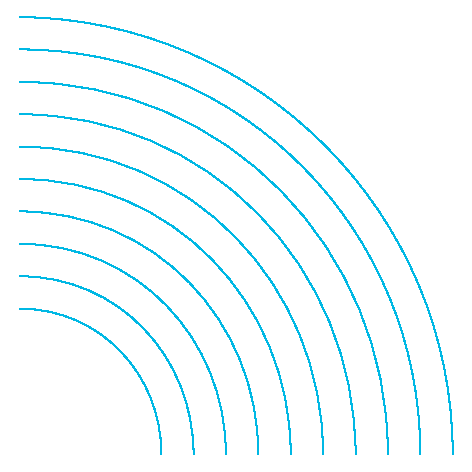
\includegraphics[width=.15\paperwidth,height=.15\paperwidth]{EETtemplateFiles/img/Simbolo_ESCOLA.pdf}\\
  
\includegraphics[width=.15\paperwidth,trim={.4cm .5cm .4cm 2.25cm},clip]{EETtemplateFiles/img/Logotipo_ESCOLA.pdf}
  \vspace*{-11pt}%
}

% MATH SYMBOLS

\newcommand{\field}[1]{\mathbb{#1}}

\DeclareMathOperator{\atan}{atan}
\DeclareMathOperator{\acos}{acos}
\DeclareMathOperator{\asin}{asin}

% \newcommand{\mb}[1]{\mathbf{#1}}


\newcommand{\A}{\mathbf{A}}
\newcommand{\B}{\mathbf{B}}
\newcommand{\Cb}{\mathbf{C}}
\newcommand{\D}{\mathbf{D}}
\newcommand{\Eb}{\mathbf{E}}
\newcommand{\F}{\mathbf{F}}
\newcommand{\Gb}{\mathbf{G}}
\newcommand{\Hb}{\mathbf{H}}
\newcommand{\I}{\mathbf{I}}
\newcommand{\J}{\mathbf{J}}
\newcommand{\Kb}{\mathbf{K}}
\newcommand{\Lb}{\mathbf{L}}
\newcommand{\M}{\mathbf{M}}
\newcommand{\N}{\mathbf{N}}
\newcommand{\Ob}{\mathbf{O}}
\newcommand{\Pb}{\mathbf{P}}
\newcommand{\Q}{\mathbf{Q}}
\newcommand{\R}{\mathbf{R}}
\newcommand{\Sb}{\mathbf{S}}
\newcommand{\T}{\mathbf{T}}
\newcommand{\U}{\mathbf{U}}
\newcommand{\V}{\mathbf{V}}
\newcommand{\W}{\mathbf{W}}
\newcommand{\X}{\mathbf{X}}
\newcommand{\Y}{\mathbf{Y}}
\newcommand{\Z}{\mathbf{Z}}
\newcommand{\Dl}{\mathbf{\boldsymbol{\Delta}}}
\newcommand{\Sg}{\mathbf{\boldsymbol{\Sigma}}}
\newcommand{\Ld}{\mathbf{\boldsymbol{\Lambda}}}
\newcommand{\Ph}{\mathbf{\boldsymbol{\Phi}}}
\newcommand{\Ps}{\mathbf{\boldsymbol{\Psi}}}
\newcommand{\Up}{\mathbf{\boldsymbol{\Upsilon}}}
\newcommand{\Xib}{\mathbf{\boldsymbol{\Xi}}}
% \newcommand{\D}{\mathbf{D}}
\newcommand{\one}{\mathbf{1}}
\newcommand{\zero}{\mathbf{0}}

\newcommand{\ab}{\mathbf{a}}
\newcommand{\bb}{\mathbf{b}}
\newcommand{\cc}{\mathbf{c}}
\newcommand{\dd}{\mathbf{d}}
\newcommand{\e}{\mathbf{e}}
\newcommand{\f}{\mathbf{f}}
\newcommand{\g}{\mathbf{g}}
\newcommand{\h}{\mathbf{h}}
\newcommand{\ib}{\mathbf{i}}
\newcommand{\jb}{\mathbf{j}}
\newcommand{\kb}{\mathbf{k}}
\newcommand{\lb}{\mathbf{\ell}}
\newcommand{\m}{\mathbf{m}}
\newcommand{\n}{\mathbf{n}}
\newcommand{\ob}{\mathbf{o}}
\newcommand{\pp}{\mathbf{p}}
\newcommand{\q}{\mathbf{q}}
\newcommand{\rr}{\mathbf{r}}
\newcommand{\s}{\mathbf{s}}
\newcommand{\uu}{\mathbf{u}}
\newcommand{\vv}{\mathbf{v}}
\newcommand{\w}{\mathbf{w}}
\newcommand{\x}{\mathbf{x}}
\newcommand{\y}{\mathbf{y}}
\newcommand{\z}{\mathbf{z}}
\newcommand{\al}{\mathbf{\boldsymbol{\alpha}}}
\newcommand{\vmu}{\mathbf{\boldsymbol{\mu}}}
\newcommand{\vlambda}{\mathbf{\boldsymbol{\lambda}}}
\newcommand{\vphi}{\mathbf{\boldsymbol{\phi}}}
\newcommand{\vpsi}{\mathbf{\boldsymbol{\psi}}}
\newcommand{\vrho}{\mathbf{\boldsymbol{\rho}}}
\newcommand{\vups}{\mathbf{\boldsymbol{\upsilon}}}
\newcommand{\vxi}{\mathbf{\boldsymbol{\xi}}}

\newcommand{\rank}{\textnormal{rank}}
% \newcommand{\trace}{\textnormal{trace}}
\newcommand{\exptr}{\textnormal{exptr}}
\newcommand{\tr}{\textnormal{tr}}
% \newcommand{\vstack}{\textnormal{vec}}
% \newcommand{\diag}{\textnormal{diag}}
\newcommand{\vstack}[1]{\Xib_{#1}}
\newcommand{\diag}[1]{\Ld_{#1}}
\newcommand{\tnsr}[2]{\underline{\mathsf{#1}}_{#2}}
\newcommand{\tmult}[1]{\underset{#1}{\times}}

\DeclareMathOperator{\Prob}{Prob}
%  |x>
\newcommand{\ket}[1]{\left\vert#1\right\rangle}
%  <x|
\newcommand{\bra}[1]{\left\langle#1\right\vert}
%  <x|y>
\newcommand{\braket}[2]{\left< #1 \vphantom{#2}\,
                        \right\vert\left.\!\vphantom{#1} #2 \right>}
%  <x|a|y>
\newcommand{\sandwich}[3]{\left< #1 \vphantom{#2 #3} \right|
                          #2 \min\left(\vphantom{#1 #2} #3 \right>}

\newcommand{\pd}[2]{\frac{\partial #1}{\partial #2}}
%  d/dt
\newcommand{\ddt}{\frac{d}{dt}}
%  D/Dx
\newcommand{\pdd}[1]{\frac{\partial}{\partial#1}}
%  |x|
\newcommand{\abs}[1]{\left\vert#1\right\vert}
%  k_{x}
\newcommand{\kv}[1]{\mathbf{k}_{#1}}
%  \textnormal{E}_{domain of integration}{variable}
\newcommand{\Ex}[2]{{\mathbb{E}_{#1}\left[#2\right]}}
\newcommand{\CEx}[3]{{\mathbb{E}_{#1}\left[#2|#3\right]}}
\newcommand{\CInf}[3]{{\textnormal{I}\left(#1;#2|#3\right)}}
\newcommand{\Inf}[2]{{\textnormal{I}\left(#1;#2\right)}}
\newcommand{\CEnt}[2]{{\textnormal{H}\left(#1|#2\right)}}
\newcommand{\Ent}[1]{{\textnormal{H}\left(#1\right)}}
\newcommand{\dCEnt}[2]{{\textnormal{h}\left(#1|#2\right)}}
\newcommand{\dEnt}[1]{{\textnormal{h}\left(#1\right)}}

\newcommand{\cmark}{\ding{51}}%
\newcommand{\xmark}{\ding{55}}%
\newcommand{\itempro}{\item[\textcolor{KYJade}{\Large \cmark}]}
\newcommand{\itemcontra}{\item[\textcolor{ARust}{\Large \xmark}]}
\newcommand\Tau{\mathcal{T}}
%Figure and format fixes


\renewcommand{\figurename}{Fig.}
\newcommand{\PESrule}{\noindent\rule{.57\columnwidth}{0.1mm}}

%theroem environments
% If using amsthm package, we need to delete these theorems before giving them our own definition. does not work for theorem
% \let\theorem\relax
\let\definition\relax
\let\lemma\relax
\let\corollary\relax
\let\example\relax
%
% \newtheorem{theorem}{Theorem}
\newtheorem{definition}{Definition}
\newtheorem{lemma}{Lemma}
\newtheorem{corollary}{Corollary}
\newtheorem{conjecture}{Conjecture}
\theoremstyle{plain}
\newtheorem{remark}{Remark}
\newtheorem{proposition}{Proposition}
\newtheorem{example}{Example}
\newtheorem{homework}{Homework}

%Colors
   \definecolor{blueH3}{rgb}{0,.5,1}
   \definecolor{blueH2}{rgb}{0,0.25,0.75}
   \definecolor{blueH1}{rgb}{0,0,0.5}   
   \definecolor{grayOldText}{rgb}{.5,.5,.5}
   \definecolor{VCobalt}{HTML}{005682}
   \definecolor{TZTeal}{HTML}{008080}
   \definecolor{TZTealfaded}{HTML}{F0FFFF}
   \definecolor{KYJade}{HTML}{008151}
   \definecolor{ARust}{HTML}{a10000}
   \definecolor{FFucsia}{HTML}{7000c3}   
   \definecolor{TAMustard}{HTML}{a1a100}
   \definecolor{Tangerine}{HTML}{d45500}
   
   
% Tikz 
% signal block diagram components
\tikzset{
    block/.style = {draw, rectangle, 
        minimum height=1cm, 
        minimum width=1.2cm, align=center},
    input/.style = {coordinate,node distance=1cm},
    output/.style = {coordinate,node distance=2cm},
    arrow/.style={draw, -latex,node distance=1.5cm},
    pinstyle/.style = {pin edge={latex-, black,node distance=1.5cm}},
    sum/.style = {draw, circle, node distance=1cm}
}
\tikzstyle{pinstyle} = [pin edge={to-,thin,black}]
\def\antenna{%
    -- +(0mm,4.0mm) -- +(2.625mm,7.5mm) -- +(-2.625mm,7.5mm) -- +(0mm,4.0mm) -- +(0mm,0mm)
}
% Overlay highlights on top of the page
\newcommand{\markOverlay}[1]{\tikz[overlay,remember picture] \node (#1) {};}
\newcommand{\drawOverlayBox}[4][]{%
    \tikz[overlay,remember picture]{%
        \coordinate (TopLeft)     at ($(#2)+(-0.4em,1.6em)$);
        \coordinate (BottomRight) at ($(#3)+(0.4em,-1.0em)$);
        %
        \path (TopLeft); \pgfgetlastxy{\XCoord}{\IgnoreCoord};
        \path (BottomRight); \pgfgetlastxy{\IgnoreCoord}{\YCoord};
        \coordinate (LabelPoint) at ($(\XCoord,\YCoord)!0.5!(BottomRight)$);
        %
        \draw [red,#1] (TopLeft) rectangle (BottomRight);
        \node [below, #1, fill=none, fill opacity=1] at (LabelPoint) {#4};
    }
}
\newcommand{\drawOverlayLine}[4][]{%
    \tikz[overlay,remember picture]{%
        \draw [red,#1] ($(#2)$) -- node{#4} ($(#3)$);
    }
}
\newcommand{\drawOverlayCircle}[4][]{%
    \tikz[overlay,remember picture]{%
        \draw [red,#1] ($(#2)$) circle (#3) node{#4};
    }
}
   
   %%%%%%%%%%%%%%%%%%%%%%%%%%%%%%%%%%%%%%%%%%%%%%%%%%%%%%%%%%%%%%%%%
%% The following definitions are to extend the LaTeX algorithmic 
%% package with SWITCH statements and one-line structures.
%% The extension is by 
%%   Prof. Farn Wang 
%%   Dept. of Electrical Engineering, 
%%   National Taiwan University. 
%% 
\newcommand{\SWITCH}[1]{\STATE \textbf{switch} (#1)}
\newcommand{\ENDSWITCH}{\STATE \textbf{end switch}}
\newcommand{\CASE}[1]{\STATE \textbf{case} #1\textbf{:} \begin{ALC@g}}
\newcommand{\ENDCASE}{\end{ALC@g}}
\newcommand{\CASELINE}[1]{\STATE \textbf{case} #1\textbf{:} }
\newcommand{\DEFAULT}{\STATE \textbf{default:} \begin{ALC@g}}
\newcommand{\ENDDEFAULT}{\end{ALC@g}}
\newcommand{\DEFAULTLINE}[1]{\STATE \textbf{default:} }
%% 
%% End of the LaTeX algorithmic package extension.

\newcounter{MYtempeqncnt}


%%%%%%%%%%%%%%%%%%%%%%%%%%%%%%%%%%%%%%%
% Commands to recall text later
%%%%%%%%%%%%%%%%%%%%%%%%%%%%%%%%%%%%%%%
\makeatletter
\newcommand\remembertext[2]{% #1 is a key, #2 is the text
  \immediate\write\@auxout{\unexpanded{\global\long\@namedef{mytext@#1}{#2}}}%
  #2%
}
%
\newcommand\recalltext[1]{%
  \ifcsname mytext@#1\endcsname
    \@nameuse{mytext@#1}%
  \else
    ``??''
  \fi
}

%%%%%%%%%%%%%%%%%%%%%%%%%%%%%%%%%%%%%%%%%%%%%%%%%%%%%%%%%%%%%%%%%%%%%%%%%%%%%%%%%%
%%% Paolo Casari: macros for automating section titling and comment formatting %%%
%%%%%%%%%%%%%%%%%%%%%%%%%%%%%%%%%%%%%%%%%%%%%%%%%%%%%%%%%%%%%%%%%%%%%%%%%%%%%%%%%%
\newcounter{myequationcnt}

\newcounter{rcnt}
\newcounter{ccnt}

\newcommand{\newreviewernopagebreak}[1]{\vspace{5em} \setcounter{ccnt}{0}\section*{\normalsize Comments of #1}\vspace{4mm}}

\newcommand{\ThisIsTheEditorNoPageBreak}{\setcounter{ccnt}{0}\section*{\Large Comments of the Editor}\vspace{3mm}}
\newcommand{\ThisIsTheEditor}{\clearpage \ThisIsTheEditorNoPageBreak}
\newcommand{\ThisIsANewReviewerNoPageBreak}[1]{\vspace{5em} \refstepcounter{rcnt}\label{r#1}\setcounter{ccnt}{0}\section*{\Large Comments of Reviewer \arabic{rcnt}}\vspace{3mm}}
\newcommand{\ThisIsANewReviewer}[1]{\clearpage\vspace{-5em} \ThisIsANewReviewerNoPageBreak{#1}}

\newcommand{\edcomment}[1]{
\begin{tcbremark}
\color{VCobalt}
    \refstepcounter{ccnt}\label{e\arabic{ccnt}}\noindent\textbf{\boldmath\emph{Comment E.\arabic{ccnt}:}} #1\vspace{0.2cm}
\end{tcbremark}
}
\newcommand{\refedcomment}[1]{E.\ref{e#1}}

\newcommand{\revcomment}[1]{
\begin{tcbremark}
\color{VCobalt}
\refstepcounter{ccnt}\label{r\arabic{rcnt}c\arabic{ccnt}}\noindent\textbf{\boldmath\emph{Comment \arabic{rcnt}.\arabic{ccnt}:}} #1\vspace{0.2cm}
\end{tcbremark}
}
\newcommand{\refrevcomment}[2]{\ref{r#1}.\ref{r#1c#2}}

% \newcommand{\ouranswer}[1]{\noindent\emph{Answer:} #1\vspace{0.6cm}}
% \newcommand{\citepap}[1]{\vspace{0.33cm}\begin{minipage}{0.05\textwidth} $\phantom{A}$  \end{minipage}\begin{minipage}{0.85\textwidth}\renewcommand{\baselinestretch}{1.15}\small \emph{#1} \end{minipage}\vspace{0.3cm}}

\newlength{\ansspace}
\addtolength{\ansspace}{0.6cm}
\newcommand{\ansbreak}{\vspace{\ansspace}}

\newlength{\stdleftskip}
\addtolength{\stdleftskip}{\leftskip}
\newlength{\stdrightskip}
\addtolength{\stdrightskip}{\rightskip}
\newlength{\citeskip}
\addtolength{\citeskip}{2em}
\newcommand{\oldbaselinestretch}{1.5}

\newcommand{\setcitepapskip}{%
    \leftskip\citeskip %
    \rightskip\citeskip %
    \renewcommand{\baselinestretch}{1.15}\small%
    \vspace{0.6em}%
    \noindent%
}

\newcommand{\resetLRmargins}{%
    \leftskip\stdleftskip %
    \rightskip\stdrightskip %
    \renewcommand{\baselinestretch}{\oldbaselinestretch}\normalsize %
    \vspace{0.6em}
}

\newcommand{\emans}{\emph{Answer:\ }}


%---------------
% LIMIAR
%---------------
%configuracion de opcions de beamer persoais, pero alleas ao estilo

% COMANDO QUE INTRODUCE UNHA DIAPOSITIVA CUN ÍNDICE NO QUE APARECEN VELADAS TÓDALAS SECCIÓNS MENOS A ACTUAL. ÚTIL PARA INTRODUCIR OS TÍPICOS ÍNDICES INTERMEDIOS.
\newcommand{\Inter}{\frame{\tableofcontents[currentsection]}}
\newcommand{\inter}{\frame{\tableofcontents[currentsection,currentsubsection]}}

% Pes de imaxe
\renewcommand{\figurename}{Fig.}
\addto\captionsenglish{\renewcommand{\figurename}{Fig.}}
\setbeamertemplate{caption}[numbered]

%ESTE PAQUETE PERMITE POÑER A BIBLIOGRAFIA AO PE DE PAXINA CON CONFIGURACIONS ESTETICAS PERSOAIS
% \usepackage[style=ieee,doi=false,isbn=false,url=true,backend=bibtex]{biblatex}
% \bibliography{./bibliografia.bib}
% \newrobustcmd*{\footfullcitenomark}{%
%   \AtNextCite{%
%     \let\thefootnote\relax 
%     \let\mkbibfootnote\mkbibfootnotetext
%     }%
%   \footfullcite}

%paquete para engadir notas de guion ao pdf
\usepackage{pgfpages}
% \setbeameroption{show only notes} 
% \setbeameroption{show notes}
% \setbeameroption{show notes on second screen=right}
% DATOS DO DOCUMENTO
\title[CDA]{Advanced Digital Communications}
\subtitle{Session 3: MIMO Spatial Multiplexing}
\author[FGC]{\underline{Felipe G\'omez-Cuba}}
\institute[GPSC]{
\begin{columns}[T]
\begin{column}{5cm}\centering
Office A-204\\
Monday-Thursday 15:00-16:30\\
\texttt{gomezcuba@gts.uvigo.es}\\
\end{column}
\end{columns}
}

\date{}

\begin{document}

% Diapositiva co título
\frame[plain]{\titlepage}

\frame[allowframebreaks]{\frametitle{Space Division Multiplexing}
    \begin{figure}
    \centering
    \caption{SDM Transmitter-Receiver Block Diagram}
    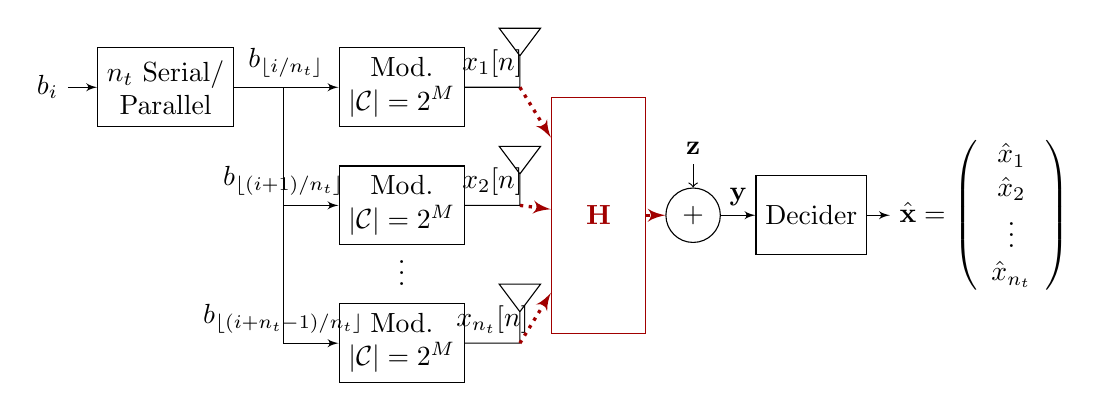
\begin{tikzpicture}[auto, node distance=1.5cm,>=latex']
        \node [pinstyle] (input)  {$b_i$};
        \node [block, right of=input] (sp) {$n_t$ Serial/\\Parallel};
        \draw[->] (input) -- (sp);
        \node [block, right of=sp, node distance=3cm] (mod1) {Mod.\\$|\mathcal{C}|=2^M$};
        \node [block, below of=mod1] (mod2) {Mod.\\$|\mathcal{C}|=2^M$};
        \node [below of=mod2, node distance=.75cm] (moddots) {$\vdots$};
        \node [block, below of=moddots, node distance=1cm] (modn) {Mod.\\$|\mathcal{C}|=2^M$};
        \draw[->] (sp) -- node{$b_{\lfloor i/n_t\rfloor}$} (mod1);
        \draw[->] (sp) -| ($(sp)!.5!(mod2)$) |- node{$b_{\lfloor (i+1)/n_t\rfloor}$}  (mod2);
        \draw[->] (sp) -| ($(sp)!.5!(mod2)$) |- node{$b_{\lfloor (i+n_t-1)/n_t\rfloor}$}  (modn);
        \node [output, right of=mod1, node distance=1.5cm] (ant1) {};
        \node [output, right of=mod2, node distance=1.5cm] (ant2) {};
        \node [output, right of=modn, node distance=1.5cm] (antn) {};
        \draw [-] (mod1) -- node {$x_1[n]$} (ant1) \antenna;            
        \draw [-] (mod2) -- node {$x_2[n]$} (ant2) \antenna;            
        \draw [-] (modn) -- node {$x_{n_t}[n]$} (antn) \antenna;
        \node [block,minimum height=3cm,ARust] (ch) at ($(ant1)!.5!(antn)+(1,0)$) {$\Hb$} ;
        \draw [->,dotted,very thick,ARust] (ant1) -- (ch);
        \draw [->,dotted,very thick,ARust] (ant2) -- (ch);
        \draw [->,dotted,very thick,ARust] (antn) -- (ch);
        \node [sum, right of=ch,node distance=1.2cm, pin={[pinstyle, pin distance=.3cm]above:$\z$}] (sum) {$+$};
        \draw [->,dotted,very thick,ARust] (ch) -- (sum);
        \node [block, right of=sum] (deco) {Decider};
        \draw [->] (sum) -- node{$\y$} (deco);
        \node [pinstyle, right of=deco,anchor=west,node distance=1cm] (soft) {$\hat{\x}=\left(\begin{array}{c}\hat{x}_1\\\hat{x}_2\\\vdots\\\hat{x}_{n_t}\end{array}\right)$};
        \draw [->] (deco) -- (soft);
    \end{tikzpicture}
    \end{figure}
    \begin{itemize}
     \item SDM greatly increases spectral efficiency $\eta=n_tM$
     \item Cannot use Gaussian Codebooks in a real circuit
     \pagebreak
     \item Define the ``M-QAM achievable rate''
        $$R_{M-QAM} =  \Inf{\x}{\y}\big|_{x_i\in\mathcal{C}_{M-QAM}}$$
     \item $R_{M-QAM}$ is similar to $C$ for some values of $P/N_o$ and $M$
        \begin{figure}
        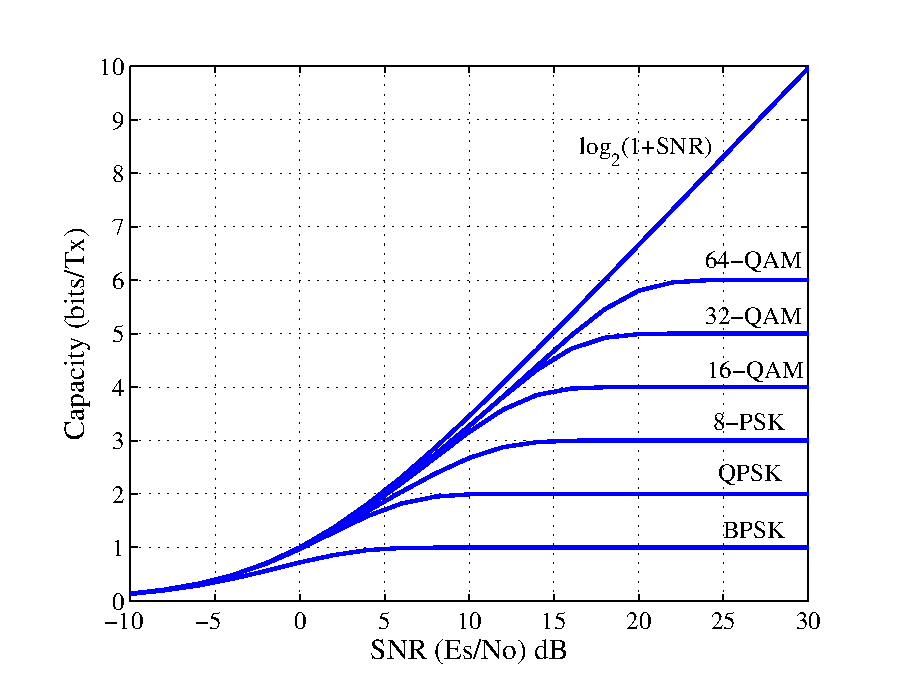
\includegraphics[width=.35\columnwidth]{capacityDiCo}
        \end{figure}
     \item Implementation: 
     \begin{itemize}
        \item Transmitter adjust $M$ vs $P/N_o$
        \item Design algorithm $\hat{\x}=\textnormal{decider}(\y)$, in general vectorial
    \end{itemize}
    \end{itemize}
}

\frame[allowframebreaks]{\frametitle{Optimal Symbol Decoding}
\begin{definition}[Decoding Error]
 Occurs if \textbf{any} of the transmitted symbols is not recovered correctly
 $$\{\hat{x}_1\neq x_1\}\cup\{\hat{x}_2\neq x_2\}\cup\dots\cup\{\hat{x}_{n_t}\neq x_{n_t}\}\equiv \hat{\x}\neq \x$$
\end{definition}
\begin{theorem}[Maximum A Posteriori (MAP) criterion]
 Minimizes the error probability over all symbols of the constellation $\hat{x}_i\in\mathcal{C}$, 
 $$\min_{\mathcal{C}^{n_t}} P(\hat{\x}\neq\x|\y)=\min_{\mathcal{C}^{n_t}} 1-P(\hat{\x}=\x|\y)\Leftrightarrow \hat{\x}_{MAP}=\arg\max_{\mathcal{C}^{n_t}} P(\x|\y)$$
\end{theorem}    
\pagebreak
\begin{definition}[Likelihood Function]
Given a random variable $Y$ with an unknown parameter $\x$, and an observation $\y$, evaluate the p.d.f. of $Y$ for different values of $\x$.
$$\mathcal{L}_{\y}(\x)=f(Y=\y|\x)$$
\end{definition}

\begin{theorem}[Maximum Likelihood (ML) criterion]
If symbols are equiprobable $P(x_i)=\frac{1}{|\mathcal{C}|}$, is equivalent to the MAP criterion and achieves minimum error probability.
$$\min P(\hat{\x}\neq \x) \Leftrightarrow \hat{\x}\stackrel{\textnormal{Bayes}}{=}\arg\max_{\x\in\mathcal{C}^{n_t}} \frac{f(\y|\x)P(\x)}{f(\y)}=\arg\max_{\x\in\mathcal{C}^{n_t}} \mathcal{L}_{\y}(\x)\cancel{\frac{1}{|\mathcal{C}|f(\y)}}$$
\end{theorem}

\begin{itemize}
 \item For the AWGN case, the p.d.f. of $(\y|\x)$ is $\mathcal{CN}(\Hb\x,\sigma_z^2\I_{n_r}$)
 \begin{equation}
    \begin{split}
     \mathcal{L}_{\y}(\x)&=f(\y|\x)\\
             &=\pi^{-n_r}\det(\sigma_z^2\I_{n_r})^{-1}e^{-(\y-\Hb\x)^H(\sigma_z^2\I_{n_r})^{-1}(\y-\Hb\x)}\\
             &=\frac{1}{(\pi\sigma_z^2)^{n_r}}e^{-\frac{\|\y-\Hb\x\|^2}{\sigma_z^2}}
    \end{split}
 \end{equation}
 \item It suffices to minimize the euclidean distance
$$\max_{\x\in\mathcal{C}^{n_t}} \mathcal{L}_{\y}(\x) \equiv \min_{\x\in\mathcal{C}^{n_t}}  \|\y-\Hb\x\|^2$$
\end{itemize}
}

\frame{\frametitle{SISO Example}
\begin{columns}
 \begin{column}{6cm}
  \begin{figure}
     \centering
     \caption{SISO $y=h_ox+z,\; x\in \mathcal{C}_{\textnormal{BPSK}}$}
     \begin{tikzpicture}
        \begin{axis}[
        width=\columnwidth,
        height=5cm,
        ymin=0,
        ymax=1.2,
        xmin=-4,
        xmax=4,
%         xtick=1,
        legend style={
            cells={anchor=west},
            legend pos=north west,
        },
        reverse legend=true,
        xtick = {-2,0,2},
        xticklabels = {$-h_o$,0,$h_o$},
        bar width=1,
    ]
     
    \addplot [thick,VCobalt] {gauss(x, 2, 1)};
    \addplot [thick,KYJade] {gauss(x, -2, 1)};
    \draw [very thick,ARust,dashed] (0,0) -- (0,1);
    \draw [->,very thick,black] (1,.3) -- (1,0);
    \node [black,anchor=south] at (1,.3) {$y$};
    \node [ARust,anchor=west] at (.3,.65) {$\hat{x}=1$};
    \node [ARust,anchor=east] at (-.3,.65) {$\hat{x}=-1$};
    \legend {$f(y|x=1)$,$f(y|x=-1)$};
    \end{axis}
     \end{tikzpicture}
    \end{figure}
 \end{column}
 \begin{column}{6cm}
  \begin{itemize}
     \item SISO ML expression
 $$\min_{\x\in\mathcal{C}^{n_t}}  \|\y-\Hb\x\|^2=\min_{x\in\mathcal{C}}  |y/h_o-x|^2$$
     \item \textit{Nearest Neighbor} criterion\\ \ \\
     \item ``Textbook'' receiver is the ML
     \begin{itemize}
     \item Automatic Gain Control
     \item Phase Locked Loop
     \item \textbf{Quantizer} $\texttt{Q}_{\mathcal{C}}()$
    \end{itemize}     
    \end{itemize}
 \end{column}
\end{columns}
}



\frame{\frametitle{Computational Complexity}

\begin{itemize}
    \item In the \textbf{estimation problem} of an arbitrary vector from continuous support  $\x\in\mathbb{C}^{n_t}$ the ML detector is \textbf{Least Squares}
    $$\hat{\x} = \arg\max_{\x\in\mathcal{X}} f(\y|\x) = \arg\min_{\x\in\mathbb{C}^{N_t}} \|\y-\Hb\x\|^2=(\Hb^H\Hb)^{-1}\Hb^H\y$$
    \item In the \textbf{decoding problem} with a discrete contellation $\x\in\mathcal{C}^{n_t}$ ML is a \textbf{NP-hard combinatorial problem}
    $$\hat{\x} = \arg\max_{\x\in\mathcal{X}} f(\y|\x) = \arg\min_{\x\in\textcolor{ARust}{\mathcal{C}^{N_t}}} \|\y-\Hb\x\|^2=\texttt{exhaustive\_search}(2^{n_tM})$$
    \item For $n_t>1$ equalizer + symbol-by-symbol decision is not ML\\ \ \\
   
    \item \textit{Gaussian Codebook} in Shannon's Theorem also NP-hard: \textbf{discrete random constellation} $\mathcal{C}$ of size $|\mathcal{C}|=2^R$ with Gaussian values
    \end{itemize}
}


\frame[allowframebreaks]{\frametitle{MIMO Receivers: Sphere Decoder (fast ML)}
\begin{columns}
 \begin{column}{6cm}
  \begin{itemize}
            \item Start with LS point of ``unconstrained ML''
            $$\textcolor{KYJade}{\overline{\x}=(\Hb^H\Hb)^{-1}\Hb^H\y}$$
            \item Measure distance to  $\overline{\x}$
             $$\|\y-\Hb\x\|^2 =  (\hat{\x}-\overline{\x})^H\textcolor{ARust}{\Hb^H\Hb}(\hat{\x}-\overline{\x})$$
            \item Test only point of $\hat\x$ close to $\overline{\x}$, within radius $\textcolor{TZTeal}{|\hat{\x}-\overline{\x}|^2\leq r}$
        \end{itemize}
 \end{column}
 \begin{column}{6cm}  
                \begin{figure}
                \caption{Sphere Demodulation}
\scalebox{.4}{
                    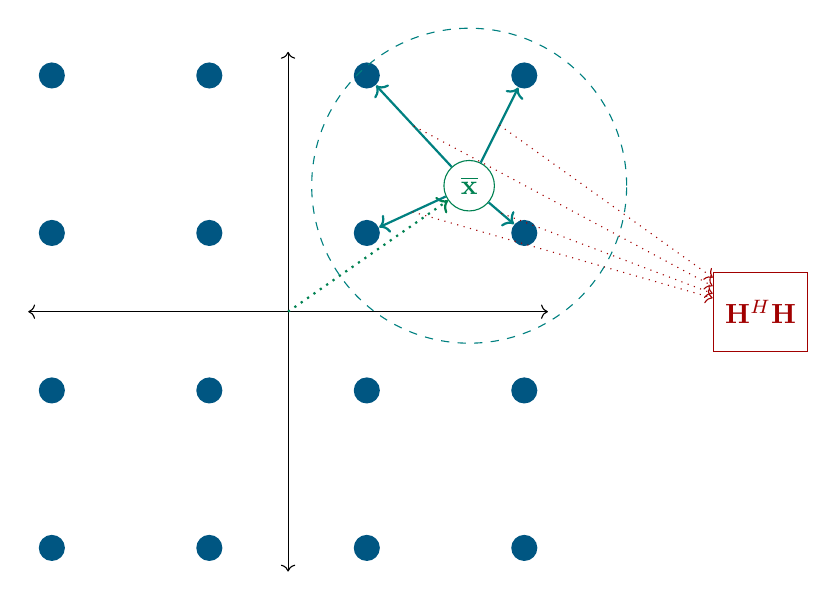
\begin{tikzpicture}
                    \draw[<->] (-3.3,0) -- (3.3,0);
                    \draw[<->] (0,-3.3) -- (0,3.3);
                    \foreach \x in {-3,-1,1,3}{
                        \foreach \y in {-3,-1,1,3}{
                            \node[circle,minimum width=.2cm,fill=VCobalt]  at (\x,\y)  (con\x\y) {};
                        }
                    }
                    \node[draw,circle,black,KYJade] at (2.3,1.6) (y) {$\overline{\mathbf{x}}$};
                    \draw[->,KYJade,thick,dotted] (0,0) -- (y);
                    \foreach \x in {1,3}{
                        \foreach \y in {1,3}{
                            \draw[->,TZTeal,thick] (y) -- node[coordinate] (mid\x\y) {} (con\x\y);
                        }
                    }
                    \draw[TZTeal,dashed] (y) circle (2cm);
                    \node[draw,block,ARust] (hb) at (6,0) {$\Hb^H\Hb$};
                    \foreach \x in {1,3}{
                        \foreach \y in {1,3}{
                            \draw[->,ARust,dotted] (mid\x\y) -- (hb);
                        }
                    }
                    \end{tikzpicture}
}
%                 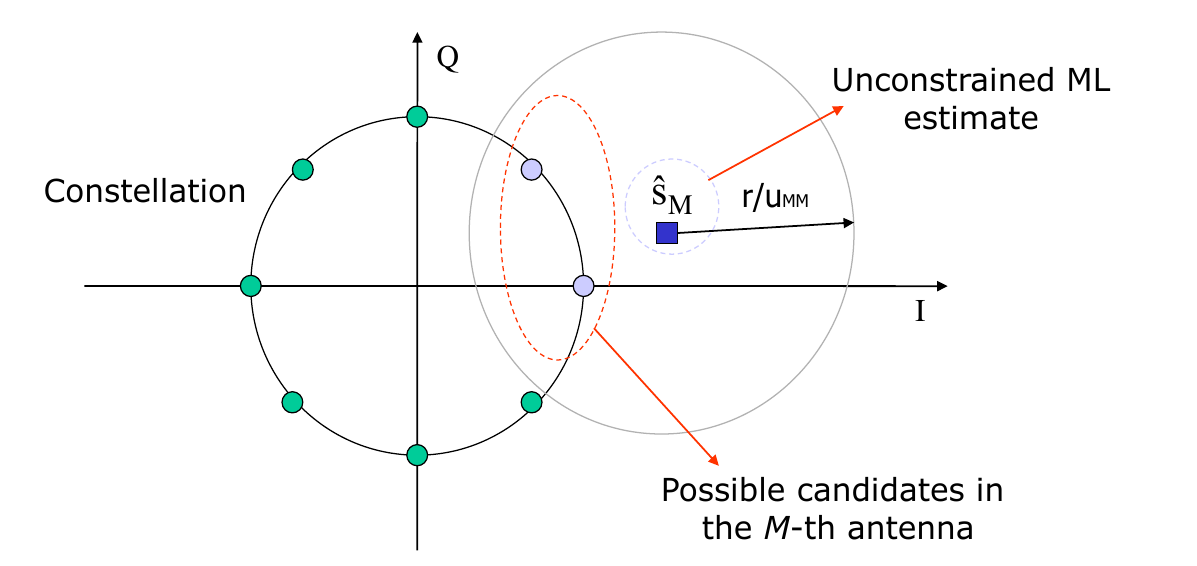
\includegraphics[width=.45\columnwidth]{sphere}
%                 \caption{Credit: Luis Castedo Ribas}
                \end{figure}
  \begin{itemize}
            \item How do we \textbf{find} which points are inside radius $r$?
        \end{itemize}
 \end{column}
\end{columns}
\pagebreak

  \begin{itemize}
            \item QR decomposition 
            $$\Hb=\Q\R\textnormal{ s.t. }\Q^H\Q=I,\;\R=\left(\begin{array}{cccc}
            r_{1,1}&r_{1,2}&\dots&r_{1,n_t}\\
            0&r_{2,2}&\dots&r_{2,n_t}\\
            \vdots&\vdots&\ddots&\vdots\\
            0&0&\dots&r_{n_t,n_t}\\
\end{array}\right)$$
%           \item Choleski decomposition 
% $$ \Hb^H\Hb=\U^H\U,\textnormal{ s.t. }\U=\left(\begin{array}{cccc}
%             u_{1,1}&u_{1,2}&\dots&u_{1,n_t}\\
%             0&u_{2,2}&\dots&u_{2,n_t}\\
%             \vdots&\vdots&\ddots&\vdots\\
%             0&0&\dots&u_{n_t,n_t}\\
% \end{array}\right)$$
            \item Recursive distance sum
$$\|\Hb(\hat{\x}-\overline{\x})\|^2=\|\R(\hat{\x}-\overline{\x})\|^2=\sum_{i=1}^{n_t}r_{i,i}^2\Big[\underset{\alpha_i}{\underbrace{\hat{x}_i-\overline{x}_i}}+\underset{\beta_i}{\underbrace{\sum_{j=i+1}^{n_t}\frac{r_{i,j}}{r_{i,i}}(\hat{x}_j-\overline{x}_j)}}\Big]$$
            \item Recursive $\beta_i=r_{i,i}\sum_{j=i+1}^{n_t}r_{i,j}\alpha_j$, starting $\beta_{n_t}=0$
            \item If $\beta_{i+1}>r\Rightarrow \|\Hb(\hat{\x}-\overline{\x})\|^2>r$
        \end{itemize}
  \begin{columns}
 \begin{column}{6cm}
 
    \setbeamercolor{postit}{fg=EETblue,bg=EETblue!10}
    \begin{beamercolorbox}[wd=\textwidth]{postit}
%     \begin{algorithm}
%     \caption{Sphere Decoder tree}
     \begin{algorithmic}[0]
      \FOR{level $i\in n_t \dots 1$}      
        \FOR{each open branch}
            \IF {$\beta_i<r$}
                \STATE Expand branch
            \ELSE
                \STATE Close branch
            \ENDIF
        \ENDFOR
      \ENDFOR
      \IF {No branches expanded}
        \STATE Increase $r$
      \ENDIF
     \end{algorithmic}
    \end{beamercolorbox}
 \end{column}
 \begin{column}{7cm}       
                \begin{figure}
                \caption{Sphere Demodulation Decision Tree}
\scalebox{.6}{
                    \begin{tikzpicture}[grow = right,
edge from parent/.style = {draw,-latex},
         label distance = .5mm,
%       every node/.style = {minimum width=2em, inner sep=2pt},
         level distance = 2.5cm,
       sibling distance = 2cm,
                        ]
                        \tikzstyle{level 1}=[sibling distance=40mm]
                        \tikzstyle{level 2}=[sibling distance=40mm]
                        \tikzstyle{level 3}=[sibling distance=20mm]
                        \tikzstyle{level 4}=[sibling distance=20mm]
                        \node[square,draw,thick,label=90:{$\beta_{n_t}=0$}] {$\emptyset$} 
                        child{
                            node[square,draw=KYJade,thick,label=90:{$\textcolor{KYJade}{\beta_{n_t-1}<r}$}] {$\hat{x}_{n_t}=1$}
                            child{
                                node[square,draw=KYJade,thick,label=90:{$\textcolor{KYJade}{\beta_{n_t-2}<r}$}] {$\hat{x}_{n_t-1}=1$}
                                child{
                                    node[square,draw=KYJade,thick,label=90:{$\textcolor{KYJade}{\beta_{n_t-3}<r}$}] {$\hat{x}_{n_t-2}=1$}
                                    child{
                                        node[square,draw=KYJade,thick,label=90:{$\textcolor{KYJade}{\beta_{n_t-4}<r}$}] {$\hat{x}_{n_t-3}=1$}
                                    } child {
                                        node[square,draw=ARust,thick,label=90:{$\textcolor{ARust}{\beta_{n_t-4}>r}$}] {$\hat{x}_{n_t-3}=0$}
                                    }
                                } child {
                                    node[square,draw=ARust,thick,label=90:{$\textcolor{ARust}{\beta_{n_t-3}>r}$}] {$\hat{x}_{n_t-2}=0$}
                                }
                            } child {
                                node[square,draw=KYJade,thick,label=90:{$\textcolor{KYJade}{\beta_{n_t-2}<r}$}] {$\hat{x}_{n_t-1}=0$}
                                child{
                                    node[square,draw=ARust,thick,label=90:{$\textcolor{ARust}{\beta_{n_t-3}>r}$}] {$\hat{x}_{n_t-2}=1$}
                                } child {
                                    node[square,draw=KYJade,thick,label=90:{$\textcolor{KYJade}{\beta_{n_t-3}<r}$}] {$\hat{x}_{n_t-2}=0$}
                                    child{
                                        node[square,draw=KYJade,thick,label=90:{$\textcolor{KYJade}{\beta_{n_t-4}<r}$}] {$\hat{x}_{n_t-3}=1$}
                                    } child {
                                        node[square,draw=ARust,thick,label=90:{$\textcolor{ARust}{\beta_{n_t-4}>r}$}] {$\hat{x}_{n_t-3}=0$}
                                    }
                                }
                            }
                        } child {
                            node[square,draw=ARust,thick,label=90:{$\textcolor{ARust}{\beta_{n_t-1}>r}$}] {$\hat{x}_{n_t}=0$}
                    };
                    \end{tikzpicture}
                    }
                \end{figure} 
 \end{column}
\end{columns}        
}




\frame[allowframebreaks]{\frametitle{MIMO Receivers: Linear Receivers}

  \begin{columns}
 \begin{column}{7cm}       
                \begin{figure}
    \centering
    \caption{Linear SDM Receiver Block Diagram}
    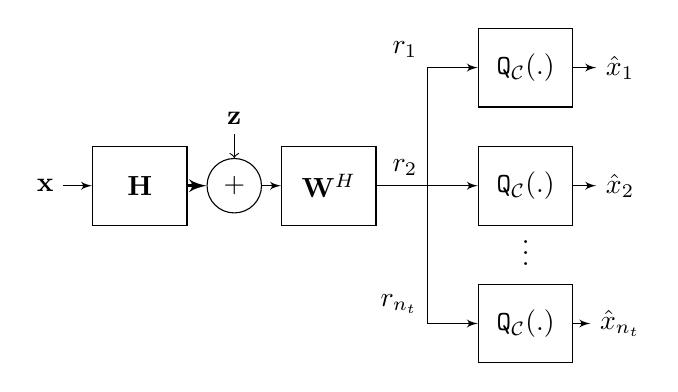
\begin{tikzpicture}[auto, node distance=1.5cm,>=latex']
        \node [pinstyle] (input)  {$\x$};
        \node [block,right of=input,node distance=1.2cm] (ch) {$\Hb$} ;
        \draw[->] (input) -- (ch);
        \node [sum, right of=ch,node distance=1.2cm, pin={[pinstyle, pin distance=.3cm]above:$\z$}] (sum) {$+$};
        \draw [->,very thick] (ch) -- (sum);
        \node [block, right of = sum,node distance=1.2cm] (wf) {$\W^H$} ;
        \draw[->] (sum) -- (wf);
        \node [block, right of=wf, node distance=2.5cm] (dmod2) {$\texttt{Q}_{\mathcal{C}}(.)$};
        \node [block, above of=dmod2] (dmod1) {$\texttt{Q}_{\mathcal{C}}(.)$};
        \node [below of=dmod2, node distance=.75cm] (dmoddots) {$\vdots$};
        \node [block, below of=dmoddots, node distance=1cm] (dmodn) {$\texttt{Q}_{\mathcal{C}}(.)$};
        \draw[->] (wf) -| ($(wf)!.5!(dmod2)$) |- node[anchor=south east]{$r_1$}  (dmod1);
        \draw[->] (wf) -- node[anchor=south east]{$r_2$} (dmod2);
        \draw[->] (wf) -| ($(wf)!.5!(dmod2)$) |- node[anchor=south east]{$r_{n_t}$}  (dmodn);
        \node [pinstyle,right of = dmod1,node distance=1.2cm] (out1)  {$\hat{x}_1$};
        \node [pinstyle,right of = dmod2,node distance=1.2cm] (out2)  {$\hat{x}_2$};
        \node [pinstyle,right of = dmodn,node distance=1.2cm] (outn)  {$\hat{x}_{n_t}$};
        \draw[->] (dmod1) -- (out1);
        \draw[->] (dmod2) -- (out2);
        \draw[->] (dmodn) -- (outn);
    \end{tikzpicture}
    \end{figure}
 \end{column}
 \begin{column}{6cm}
 \begin{itemize}
        \item Linear matrix filter 
        $$\rr=\W^H\y=\left(\begin{array}{c}r_1\\r_2\\\vdots\\r_{n_t}\end{array}\right)$$
        \item Design $\W$ so that $r_i$ associated to one $x_i$\\ \ \\
        \item Symbol-by-symbol decision
        $$\hat{x}_i=\texttt{Q}_{\mathcal{C}}(r_i)=\arg\min_{x'\in\mathcal{C}}|r_i-x'|$$
     \end{itemize}
 \end{column}
\end{columns}  

  \begin{columns}
 \begin{column}{7cm}       
                \begin{figure}
    \centering
    \caption{Linear SDM Receiver Block Diagram}
    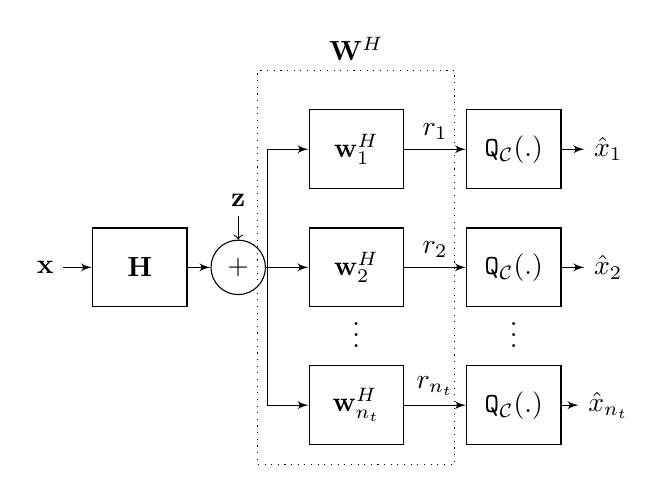
\begin{tikzpicture}[auto, node distance=1.5cm,>=latex']
        \node [pinstyle] (input)  {$\x$};
        \node [block,right of=input,node distance=1.2cm] (ch) {$\Hb$} ;
        \draw[->] (input) -- (ch);
        \node [sum, right of=ch,node distance=1.25cm, pin={[pinstyle, pin distance=.3cm]above:$\z$}] (sum) {$+$};
        \draw [->] (ch) -- (sum);
        \node [block, right of=sum, node distance=1.5cm] (w2) {$\w_2^H$};
        \node [block, above of=w2] (w1) {$\w_1^H$};
        \node [below of=w2, node distance=.75cm] (wdots) {$\vdots$};
        \node [block, below of=wdots, node distance=1cm] (wn) {$\w_{n_t}^H$};
        \draw[->] (sum) -| ($(sum)!.25!(w2)$) |-  (w1);
        \draw[->] (sum) -- (w2);
        \draw[->] (sum) -| ($(sum)!.25!(w2)$) |-  (wn);
        \node [block,dotted,minimum height=5cm,minimum width=2.5cm,label=90:{$\W^H$}] at (w2) (wf) {} ;
        \node [block, right of=w2, node distance=2cm] (dmod2) {$\texttt{Q}_{\mathcal{C}}(.)$};
        \node [block, above of=dmod2] (dmod1) {$\texttt{Q}_{\mathcal{C}}(.)$};
        \node [below of=dmod2, node distance=.75cm] (dmoddots) {$\vdots$};
        \node [block, below of=dmoddots, node distance=1cm] (dmodn) {$\texttt{Q}_{\mathcal{C}}(.)$};
        \draw[->] (w1) -- node[anchor=south]{$r_1$}  (dmod1);
        \draw[->] (w2) -- node[anchor=south]{$r_2$} (dmod2);
        \draw[->] (wn) -- node[anchor=south]{$r_{n_t}$}  (dmodn);
        \node [pinstyle,right of = dmod1,node distance=1.2cm] (out1)  {$\hat{x}_1$};
        \node [pinstyle,right of = dmod2,node distance=1.2cm] (out2)  {$\hat{x}_2$};
        \node [pinstyle,right of = dmodn,node distance=1.2cm] (outn)  {$\hat{x}_{n_t}$};
        \draw[->] (dmod1) -- (out1);
        \draw[->] (dmod2) -- (out2);
        \draw[->] (dmodn) -- (outn);
    \end{tikzpicture} 
    \end{figure}
 \end{column}
 \begin{column}{6cm}
 \begin{itemize}
    \item Row-column matrix product
        $$\W^H\Hb=\left[\begin{array}{c}\w_1^H\\\hline\w_2^H\\\hline\vdots\\\hline\w_{n_t}^H\end{array}\right]\left[\h_1|\h_2|\dots|\h_{n_t}\right]$$
    \item Equivalent channel
    $$r_i=\underset{\textnormal{Data}}{\underbrace{\w_i^H\h_i x_i}} +\underset{\textnormal{Inter Sym. Interf.}}{\underbrace{\sum_{j\neq i}\w_i^H\h_j x_j}} +\underset{\textnormal{Noise}}{\underbrace{\w_i^H\z}}$$
     \end{itemize}
 \end{column}
\end{columns} 
\begin{definition}[Signal to Interference plus Noise Ratio (SINR)]
 $ \textnormal{SINR}_i=\gamma_i=\frac{\Ex{}{ \|\w_i^H\h_i x_i\|^2}}{\Ex{}{ \|\w_i^H\h_j x_j\|^2}+\Ex{}{ \|\w_i^H\z_i\|^2}}=\frac{\|\w_i^H\h_i\|^2\frac{P}{n_t}}{\sum_{j\neq i}\|\w_i^H\h_j\|^2\frac{P}{n_t}+\cancel{\|\w_i\|^2}^{1}\sigma^2}$
\end{definition}
\begin{theorem}[Treating Interference as Noise (TIN)]
 The Gaussian distribution is the worst (i.e. lowest ``achievable rate'') of all the possible random noise distributions of the same variance
 $$R_{TIN_i}=\Inf{r_i}{x_i}\geq \log\left(1+\gamma_i\right)$$
 Assuming Gaussian interference, the AWGN BER formulas can be used
 \begin{table}
 \begin{tabular}{c|ccc}
  $\mathcal{C}$& QPSK & MPSK & M-QAM\\\hline
  $BER_{TIN}^{(i)}\approx$ & $\mathcal{Q}(\sqrt{2\gamma_i})$ & $\frac{2}{\log_2 M}\mathcal{Q}(\sqrt{2\gamma_i}\sin(\pi/M))$& $\frac{2(\sqrt{M}-1)}{\sqrt{M}\log_2 M}\mathcal{Q}(\sqrt{\frac{3\gamma_i}{(M-1)}})$ \\
 \end{tabular}
 \end{table}
\end{theorem}

 
\begin{figure}
    \centering
    \caption{Linear SDM Matched Filter Receiver}
    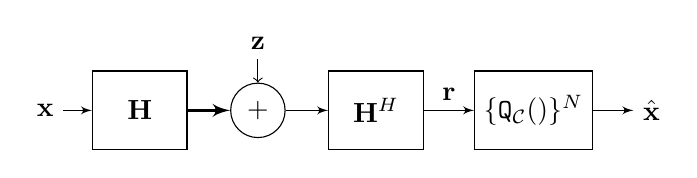
\begin{tikzpicture}[auto, node distance=2cm,>=latex']
        \node [pinstyle] (input)  {$\x$};
        \node [block,right of=input,node distance=1.2cm] (ch) {$\Hb$} ;
        \draw[->] (input) -- (ch);
        \node [sum, right of=ch,node distance=1.5cm, pin={[pinstyle, pin distance=.3cm]above:$\z$}] (sum) {$+$};
        \draw [->,very thick] (ch) -- (sum);
        \node [block, right of = sum,node distance=1.5cm] (wf) {$\Hb^H$} ;
        \draw[->] (sum) -- (wf);
        \node [block, right of=wf] (qtz) {$\{\texttt{Q}_{\mathcal{C}}()\}^N$};
        \draw[->] (wf) -- node {$\rr$} (qtz);
        \node [pinstyle,right of = qtz,node distance=1.5cm] (out)  {$\hat{\x}$};
        \draw[->] (qtz) -- (out);
    \end{tikzpicture}
    \end{figure}
    \begin{itemize}
     \item \textbf{Matched filter} maximizes SNR $\W^H=\Hb^H\to \w_i^H=\h_i^H\to \max \frac{|\w_i^H\h|^2}{\|\w_i\|^2\sigma^2}\frac{P}{n_t}$
     \vspace{-.2in}
     $$\gamma_i=\frac{\left|\|\h_i\|^2\right|^2\frac{P}{n_t}}{\sum_{j\neq i}|\h_i^H\h_j|^2\frac{P}{n_t}+\|\h_i\|^2\sigma^2}=\frac{\|\h_i\|^2}{\frac{\|\h_i^H\Hb\|^2-\|\h_i\|^2}{\|\h_i\|^2}+\frac{n_t\sigma^2}{P}}\;\neq $$
%      $$SNR=\frac{\|\Hb^H\Hb\|^2P}{\|\Hb\|^2n_t\sigma^2_1}=\frac{P\left(\sum_{i=1}^{n_t} \frac{\lambda_i^2}{\left(\sum_{i=1}^{n_t} \lambda_i^2\right)}\right)}{\sigma^2_z}$$
     \item MRC optimum in SIMO ($n_t=1$) and orthogonal channels $\h_i^H\h_j= 0$
     \item In \textit{Massive MIMO} $\h_i^H\h_j\approx 0$
    \end{itemize}      
    
    
 
\begin{figure}
    \centering
    \caption{Linear SDM Zero Forcing Receiver}
    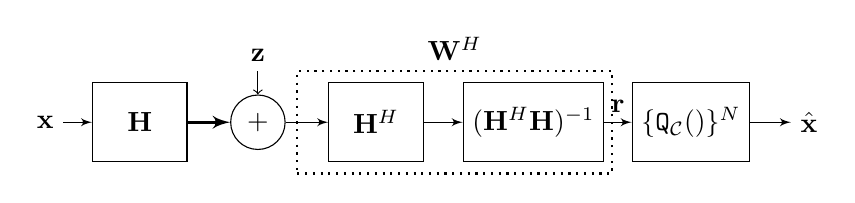
\begin{tikzpicture}[auto, node distance=2cm,>=latex']
        \node [pinstyle] (input)  {$\x$};
        \node [block,right of=input,node distance=1.2cm] (ch) {$\Hb$} ;
        \draw[->] (input) -- (ch);
        \node [sum, right of=ch,node distance=1.5cm, pin={[pinstyle, pin distance=.3cm]above:$\z$}] (sum) {$+$};
        \draw [->,very thick] (ch) -- (sum);
        \node [block, right of = sum,node distance=1.5cm] (mf) {$\Hb^H$} ;
        \draw[->] (sum) -- (mf);
        \node [block, right of = mf,node distance=2cm] (if) {$(\Hb^H\Hb)^{-1}$} ;
        \draw[->] (mf) -- (if);
        \node [block, right of=if] (qtz) {$\{\texttt{Q}_{\mathcal{C}}()\}^N$};        
        \node [block,dotted,thick,minimum height=1.3cm,minimum width=4cm,label=90:{$\W^H$}] at ($(mf)!.5!(if)$) (wf) {} ;
        \draw[->] (if) -- node {$\rr$} (qtz);
        \node [pinstyle,right of = qtz,node distance=1.5cm] (out)  {$\hat{\x}$};
        \draw[->] (qtz) -- (out);
    \end{tikzpicture}
    \end{figure}
    \vspace{-.1in}
    \begin{itemize}
     \item \textbf{Zero Forcing Equalizer} eliminates interference $\W^H\Hb=\I \to\rr=\x+\W^H\z$
     \item Pseudoinverse $\W^H=(\Hb^{H}\Hb)^{-1}\Hb^H=\arg\min \Ex{}{\|\W^H\z\|^2} \textnormal{ s.t. }\W^H\Hb=\I$ 
     
     $$SNR=\frac{\Ex{}{\|\x\|^2}}{\Ex{}{\|\W^H\z\|^2}}=\frac{P}{\tr\{\left(\Hb\Hb^H\right)^{-1}\}\sigma_z^2}=\frac{P}{\sigma_z^2\left(\sum_{i=1}^{n_t}\frac{1}{\lambda_1}\right)}$$
     \item $\w_i$'s are ``decorrelators''
     \item Optimum in high-SNR regime 
    \end{itemize}
    \pagebreak
    
    \vspace{-.1in}
    \begin{definition}[Mean Squared Error]
     $$\ev=\x-\rr\to\Ex{}{\|\ev\|^2}=\Ex{}{\|\x-\rr\|^2}=\Ex{}{\|\x-\W^H\y\|^2}$$
    \end{definition}
    \begin{itemize}
     \item Distributive properties
     \begin{equation*}
        \begin{split}
        \Ex{}{\|\ev\|^2}&=\Ex{}{(\x-\W^H\Hb\x-\W^H\z)^H(\x-\W^H\Hb\x-\W^H\z)^H)}\\
                        &=\Ex{}{(\x^H(\I-\W^H\Hb)^H(\I-\W^H\Hb)\x}+\Ex{}{(\z^H\W\W^H\z}\\
                        &\qquad+\cancel{\Ex{}{\x^H}}(\I-\W^H\Hb)^H\cancel{\Ex{}{\z}}+\cancel{\Ex{}{\z^H}}(\I-\W^H\Hb)\cancel{\Ex{}{\x}}\\
        \end{split}
     \end{equation*}
     \item Rotation of the trace $\ab^H\B\cc=\tr\{\ab^H\B\cc\}=\tr\{\cc\ab^H\B\}$
     $$\Ex{}{\|\ev\|^2}=\Ex{}{\tr\{\x\x^H(\I-\W^H\Hb)^H(\I-\W^H\Hb\}}+\Ex{}{\tr\{\z\z^H\W\W^H\}}$$
     \item Average and trace are linear operators
     $$\Ex{}{\|\ev\|^2}=\tr\{\K_{\x}(\I-\W^H\Hb)^H(\I-\W^H\Hb\}+\tr\{\K_{\z}\W\W^H\}$$
     \item I.i.d. noise and data 
     $$\Ex{}{\|\ev\|^2}=\frac{P}{n_t}\left(\tr\{\I_{n_t}\}-\tr\{\Hb^H\W\}-\tr\{\W^H\Hb\}+\tr\{\W^H\Hb\Hb^H\W\}\right)+\sigma_z^2\tr\{\W\W^H\}\}$$
     \item Group the terms of a 2nd order ``polynomial'' (and $\A^H+\A=2\Re\{\A\}$)
     $$\Ex{}{\|\ev\|^2}==P+\frac{P}{n_t}\underset{\mathscr{F}(\W)}{\underbrace{\left[-2\tr\{\Re\{\Hb^H\W\}\}+\tr\left\{\W^H\left(\Hb\Hb^H+\frac{n_t\sigma_z}{P}\I_{n_r}\right)\W\right\}\right]}}$$
     \item Gradient equal to zero
       \begin{equation*}
        \begin{split}
        \zero &= \nabla \mathscr{F}(\W) =-\Hb^H+\W^H\left(\Hb\Hb^H+\frac{n_t\sigma_z}{P}\I\right)\\
                        \Hb^H&=\W^H\left(\Hb\Hb^H+\frac{n_t\sigma_z}{P}\I_{n_r}\right)\\
                        \W^H&=\Hb^H\left(\Hb\Hb^H+\frac{n_t\sigma_z}{P}\I_{n_r}\right)^{-1}\\
        \end{split}
        \end{equation*}
     \item Matrix Inversion Lemma
     $$\underset{n\times m}{\underbrace{\B}}\left(\I_{n}+\A\B\right)^{-1}=\left(\I_{m}+\B\A\right)^{-1}\B\to \W^H=\left(\Hb^H\Hb+\frac{n_t\sigma_z}{P}\I_{n_t}\right)^{-1}\Hb^H$$
    \end{itemize}
    
\begin{figure}
    \centering
    \caption{Linear SDM MMSE Receiver}
    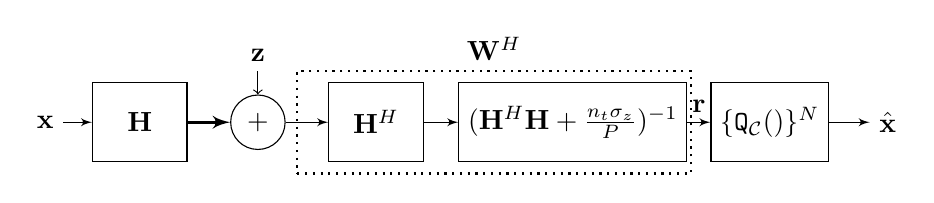
\begin{tikzpicture}[auto, node distance=2cm,>=latex']
        \node [pinstyle] (input)  {$\x$};
        \node [block,right of=input,node distance=1.2cm] (ch) {$\Hb$} ;
        \draw[->] (input) -- (ch);
        \node [sum, right of=ch,node distance=1.5cm, pin={[pinstyle, pin distance=.3cm]above:$\z$}] (sum) {$+$};
        \draw [->,very thick] (ch) -- (sum);
        \node [block, right of = sum,node distance=1.5cm] (mf) {$\Hb^H$} ;
        \draw[->] (sum) -- (mf);
        \node [block, right of = mf,node distance=2.5cm] (if) {$(\Hb^H\Hb+\frac{n_t\sigma_z}{P})^{-1}$} ;
        \draw[->] (mf) -- (if);
        \node [block, right of=if,node distance=2.5cm] (qtz) {$\{\texttt{Q}_{\mathcal{C}}()\}^N$};        
        \node [block,dotted,thick,minimum height=1.3cm,minimum width=5cm,label=90:{$\W^H$}] at ($(mf)!.6!(if)$) (wf) {} ;
        \draw[->] (if) -- node {$\rr$} (qtz);
        \node [pinstyle,right of = qtz,node distance=1.5cm] (out)  {$\hat{\x}$};
        \draw[->] (qtz) -- (out);
    \end{tikzpicture}
    \end{figure}
    \vspace{-.1in}
    \begin{itemize}
     \item \textbf{Minimum MSE Equalizer} maximizes the SINR     
     $$\rr=\x+\ev\to \textnormal{SINR}=\frac{\Ex{}{\|\x\|^2}}{\Ex{}{\|\ev\|^2}}\geq \frac{P}{\textnormal{MMSE}}$$
     $$\textnormal{SINR}_{\textnormal{MMSE}}=\frac{P}{\tr\{\left(\Hb\Hb^H+\frac{n_t\sigma_z^2}{P}\I\right)^{-1}\}\sigma_z^2}=\frac{P}{\sigma_z^2\left(\sum_{i=1}^{n_t}\frac{1}{\lambda_1+\frac{n_t\sigma_z^2}{P}}\right)}>\textnormal{SNR}_{ZF}$$
    \end{itemize}   
}
% 
\frame[allowframebreaks]{\frametitle{MIMO Receivers: Linear Feedback}
    \begin{figure}
    \centering
    \caption{General Linear SDM Receivers Structure}
    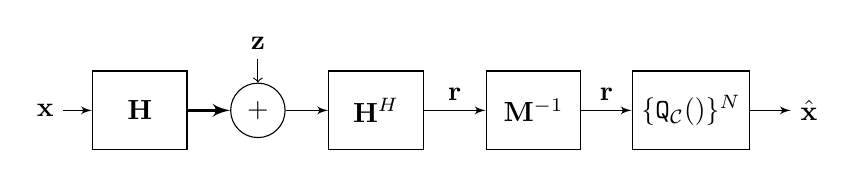
\begin{tikzpicture}[auto, node distance=2cm,>=latex']
        \node [pinstyle] (input)  {$\x$};
        \node [block,right of=input,node distance=1.2cm] (ch) {$\Hb$} ;
        \draw[->] (input) -- (ch);
        \node [sum, right of=ch,node distance=1.5cm, pin={[pinstyle, pin distance=.3cm]above:$\z$}] (sum) {$+$};
        \draw [->,very thick] (ch) -- (sum);
        \node [block, right of = sum,node distance=1.5cm] (mf) {$\Hb^H$} ;
        \draw[->] (sum) -- (mf);
        \node [block, right of = mf,node distance=2cm] (if) {$\M^{-1}$} ;
        \draw[->] (mf) -- node {$\rr$} (if);
        \node [block, right of=if] (qtz) {$\{\texttt{Q}_{\mathcal{C}}()\}^N$};
        \draw[->] (if) -- node {$\rr$} (qtz);
        \node [pinstyle,right of = qtz,node distance=1.5cm] (out)  {$\hat{\x}$};
        \draw[->] (qtz) -- (out);
    \end{tikzpicture}
    \end{figure}
    
    \begin{itemize}
     \item ``Denoising'' Matched filter $\rr_{MF}=\Hb^H\y$
        \begin{itemize}
        \item Removes noise $\perp_{\Hb}$
        \item Leaves interference
        \end{itemize}
     \item Decorrelation filter $\rr=\M^{-1}\rr_{MF}$
        \begin{itemize}
        \item Removes interference
        \item Does not change noise
        \end{itemize}
    \end{itemize}
\pagebreak
 \begin{itemize}
  \item Cholesky matrix inverse algorithm
    \begin{enumerate}
       \item Solve $\Lb^H\Deltab\vv_{aux}=\rr_{MF}$ with $\rr_{MF}=\Hb^H\y$
       \item Solve $\Lb\rr=\vv_{aux}$
    \end{enumerate}
  
      \begin{figure}
    \centering
%     \caption{Linear SDM Receiver}
\vspace{-.1in}
    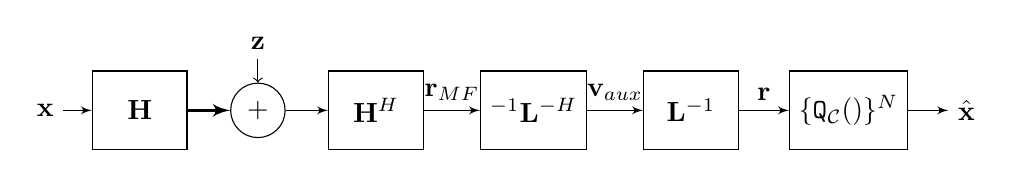
\begin{tikzpicture}[auto, node distance=2cm,>=latex']
        \node [pinstyle] (input)  {$\x$};
        \node [block,right of=input,node distance=1.2cm] (ch) {$\Hb$} ;
        \draw[->] (input) -- (ch);
        \node [sum, right of=ch,node distance=1.5cm, pin={[pinstyle, pin distance=.3cm]above:$\z$}] (sum) {$+$};
        \draw [->,very thick] (ch) -- (sum);
        \node [block, right of = sum,node distance=1.5cm] (mf) {$\Hb^H$} ;
        \draw[->] (sum) -- (mf);
        \node [block, right of = mf,node distance=2cm] (lf) {$\Deltab^{-1}\Lb^{-H}$} ;
        \draw[->] (mf) -- node {$\rr_{MF}$} (lf);
        \node [block, right of = lf,node distance=2cm] (if) {$\Lb^{-1}$} ;
        \draw[->] (lf) -- node {$\vv_{aux}$} (if);
        \node [block, right of=if] (qtz) {$\{\texttt{Q}_{\mathcal{C}}()\}^N$};
        \draw[->] (if) -- node {$\rr$} (qtz);
        \node [pinstyle,right of = qtz,node distance=1.5cm] (out)  {$\hat{\x}$};
        \draw[->] (qtz) -- (out);
    \end{tikzpicture}
    \end{figure}
\vspace{-.1in}
\begin{definition}[Cholesky Decomposition]
Hermitian matrix $\M=\Lb^H\Deltab\Lb$ where
$$\Lb=\left(\begin{array}{cccc}
            1&0&\dots&0\\
            \ell_{2,1}&1&\dots&0\\
            \vdots&\vdots&\ddots&\vdots\\
            \ell_{n_t,1}&\ell_{n_t,2}&\dots&1\\
\end{array}\right),\;\Deltab_{n_t}=\left(\begin{array}{cccc}
 \delta_1&0&\dots&0\\
 0&\delta_2&\dots&0\\
 \vdots&\vdots&\ddots&\vdots\\
 0&0&\dots&\delta_{n_t}\\
\end{array}\right)$$
\end{definition}
      
  \item Taylor series of matrix inverse $\M^{-1}=\prod_{n=1}^{\infty}(\I-\M)^n$
    \begin{figure}
    \centering
    \caption{Recursive infinite filter $\rr^{(n+1)}=\rr_{MF}+(\I-\M)\rr^{(n)}$}
\vspace{-.2in}
    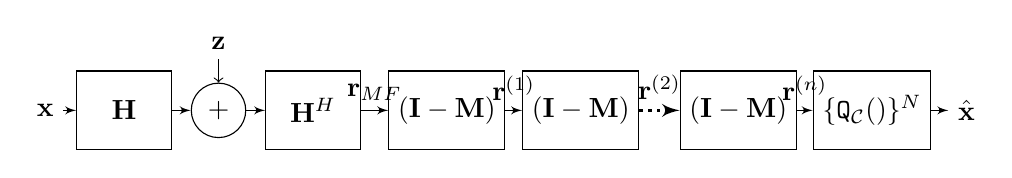
\begin{tikzpicture}[auto, node distance=2cm,>=latex']
        \node [pinstyle] (input)  {$\x$};
        \node [block,right of=input,node distance=1cm] (ch) {$\Hb$} ;
        \draw[->] (input) -- (ch);
        \node [sum, right of=ch,node distance=1.2cm, pin={[pinstyle, pin distance=.3cm]above:$\z$}] (sum) {$+$};
        \draw [->] (ch) -- (sum);
        \node [block, right of = sum,node distance=1.2cm] (mf) {$\Hb^H$} ;
        \draw[->] (sum) -- (mf);
        \node [block, right of = mf,node distance=1.7cm] (lf1) {$(\I-\M)$} ;
        \draw[->] (mf) -- node {$\rr_{MF}$} (lf1);
        \node [block, right of = lf1,node distance=1.7cm] (lf2) {$(\I-\M)$} ;
        \draw[->] (lf1) -- node {$\rr^{(1)}$} (lf2);
        \node [block, right of = lf2,node distance=2cm] (lfn) {$(\I-\M)$} ;
        \draw[->,dotted,very thick] (lf2) -- node {$\rr^{(2)}$} (lfn);
        \node [block, right of=lfn,node distance=1.7cm] (qtz) {$\{\texttt{Q}_{\mathcal{C}}()\}^N$};
        \draw[->] (lfn) -- node {$\rr^{(n)}$} (qtz);
        \node [pinstyle,right of = qtz,node distance=1.2cm] (out)  {$\hat{\x}$};
        \draw[->] (qtz) -- (out);
    \end{tikzpicture}
    \end{figure}
\vspace{-.1in}
        
    \begin{figure}
    \centering
    \caption{Infinite Impulse Response Filter}
    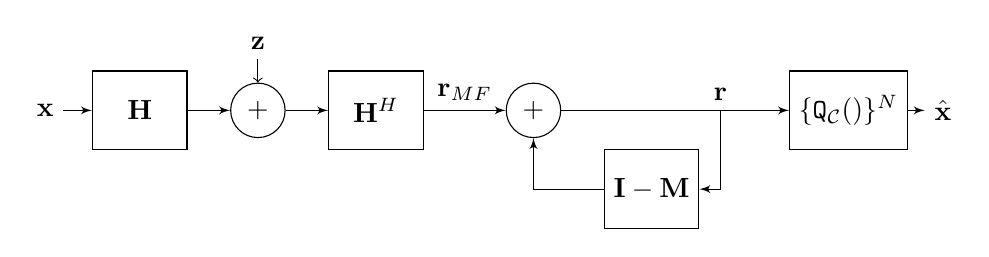
\begin{tikzpicture}[auto, node distance=2cm,>=latex']
        \node [pinstyle] (input)  {$\x$};
        \node [block,right of=input,node distance=1.2cm] (ch) {$\Hb$} ;
        \draw[->] (input) -- (ch);
        \node [sum, right of=ch, node distance=1.5cm, pin={[pinstyle, pin distance=.3cm]above:$\z$}] (sum) {$+$};
        \draw [->] (ch) -- (sum);
        \node [block, right of = sum, node distance=1.5cm] (mf) {$\Hb^H$} ;
        \draw [->] (sum) -- (mf);
        \node [sum, right of=mf, node distance=2cm] (sum2) {$+$};
        \draw [->] (mf) -- node {$\rr_{MF}$}(sum2);
        \node [coordinate, right of = sum2, node distance=1.5cm] (nofilt) {};
        \node [block, right of=nofilt, node distance=2.5cm] (qtz) {$\{\texttt{Q}_{\mathcal{C}}()\}^N$};
        \draw[->] (sum2) -- (nofilt) -- node [name=tap]{$\rr$} (qtz);
        \node [pinstyle,right of = qtz,node distance=1.2cm] (out)  {$\hat{\x}$};
        \draw[->] (qtz) -- (out);
        \node [block, below of=nofilt, node distance=1cm] (feedback) {$\I-\M$};
        \draw [->] (tap) |- node [above,pos=0.79] {} (feedback) ;
        \draw [->] (feedback) -| node[pos=0.99] {} node [near end] {} (sum2);
    \end{tikzpicture}
    \end{figure}
 \end{itemize}
}



\frame[allowframebreaks]{\frametitle{Non-linear MIMO Receivers: Decision Feedback}
\begin{figure}
    \centering
    \caption{Parallel Interference Cancelling}
\vspace{-.2in}
    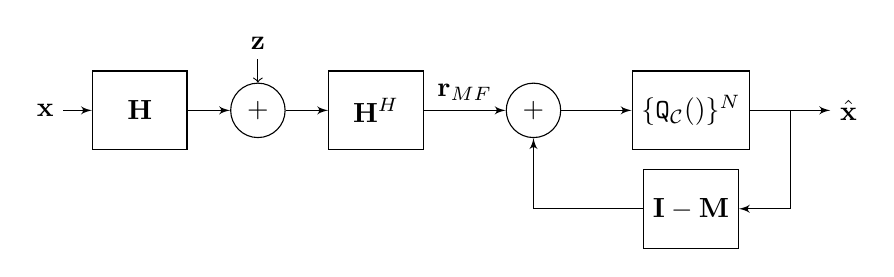
\begin{tikzpicture}[auto, node distance=2cm,>=latex']
        \node [pinstyle] (input)  {$\x$};
        \node [block,right of=input,node distance=1.2cm] (ch) {$\Hb$} ;
        \draw[->] (input) -- (ch);
        \node [sum, right of=ch, node distance=1.5cm, pin={[pinstyle, pin distance=.3cm]above:$\z$}] (sum) {$+$};
        \draw [->] (ch) -- (sum);
        \node [block, right of = sum, node distance=1.5cm] (mf) {$\Hb^H$} ;
        \draw [->] (sum) -- (mf);
        \node [sum, right of=mf, node distance=2cm] (sum2) {$+$};
        \draw [->] (mf) -- node {$\rr_{MF}$}(sum2);
        \node [block, right of = sum2, node distance=2cm] (qtz) {$\{\texttt{Q}_{\mathcal{C}}()\}^N$};
        \draw[->] (sum2) -- (qtz);
        \node [pinstyle,right of = qtz,node distance=2cm] (out)  {$\hat{\x}$};
        \draw[->] (qtz) -- node [name=tap] {} (out);
        \node [block, below of=qtz, node distance=1.25cm] (feedback) {$\I-\M$};
        \draw [->] (tap) |- node [above,pos=0.79] {} (feedback) ;
        \draw [->] (feedback) -| node[pos=0.99] {} node [near end] {} (sum2);
    \end{tikzpicture}
    \end{figure}
\begin{figure}
    \centering
    \caption{Successive Interference Cancelling (Cholesky)}
\vspace{-.2in}
    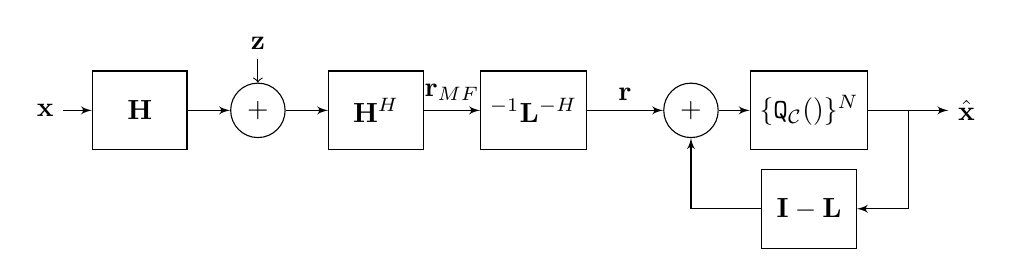
\begin{tikzpicture}[auto, node distance=2cm,>=latex']
        \node [pinstyle] (input)  {$\x$};
        \node [block,right of=input,node distance=1.2cm] (ch) {$\Hb$} ;
        \draw[->] (input) -- (ch);
        \node [sum, right of=ch, node distance=1.5cm, pin={[pinstyle, pin distance=.3cm]above:$\z$}] (sum) {$+$};
        \draw [->] (ch) -- (sum);
        \node [block, right of = sum, node distance=1.5cm] (mf) {$\Hb^H$} ;
        \draw [->] (sum) -- (mf);
        \node [block, right of = mf, node distance=2cm] (ff) {$\Deltab^{-1}\Lb^{-H}$} ;
        \draw [->] (mf) -- node {$\rr_{MF}$}(ff);
        \node [sum, right of=ff, node distance=2cm] (sum2) {$+$};
        \draw [->] (ff) -- node {$\rr$} (sum2);
        \node [block, right of = sum2, node distance=1.5cm] (qtz) {$\{\texttt{Q}_{\mathcal{C}}()\}^N$};
        \draw[->] (sum2) -- (qtz);
        \node [pinstyle,right of = qtz,node distance=2cm] (out)  {$\hat{\x}$};
        \draw[->] (qtz) -- node [name=tap] {} (out);
        \node [block, below of=qtz, node distance=1.25cm] (feedback) {$\I-\Lb$};
        \draw [->] (tap) |- node [above,pos=0.79] {} (feedback) ;
        \draw [->] (feedback) -| node[pos=0.99] {} node [near end] {} (sum2);
    \end{tikzpicture}
    \end{figure}
    \pagebreak
     \begin{itemize}
     \item QR decomposition of $\Hb=\Q\R$ (Lower triangular $\R$)\\ \ \\
     \item Choleski decomposition $\Hb^H\Hb=\Lb^H\Deltab\Lb$ ($\R=\Deltab^{\frac{1}{2}}\Lb$)\\ \ \\
     \item Triangular equivalent channel
        $$\rr=\Deltab^{-\frac{1}{2}}\Q^H\y=\Deltab^{-\frac{1}{2}}\R\x+\Deltab^{-\frac{1}{2}}\Q\z=\Lb\x+\Deltab^{-\frac{1}{2}}\z'$$
    \end{itemize}
        
\begin{figure}
    \centering
    \caption{Successive Interference Cancelling (QR)}
\vspace{-.2in}
    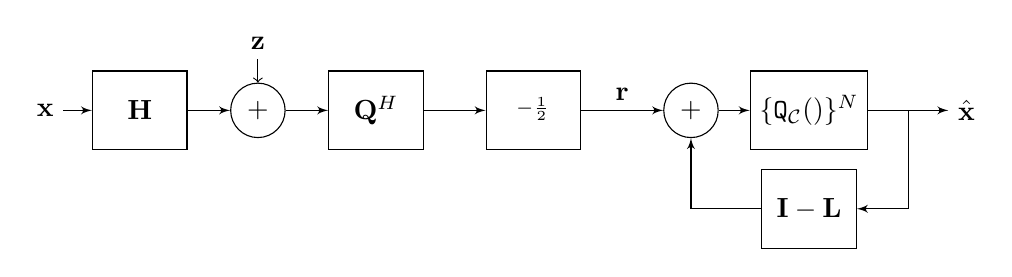
\begin{tikzpicture}[auto, node distance=2cm,>=latex']
        \node [pinstyle] (input)  {$\x$};
        \node [block,right of=input,node distance=1.2cm] (ch) {$\Hb$} ;
        \draw[->] (input) -- (ch);
        \node [sum, right of=ch, node distance=1.5cm, pin={[pinstyle, pin distance=.3cm]above:$\z$}] (sum) {$+$};
        \draw [->] (ch) -- (sum);
        \node [block, right of = sum, node distance=1.5cm] (mf) {$\Q^H$} ;
        \draw [->] (sum) -- (mf);
        \node [block, right of = mf, node distance=2cm] (ff) {$\Deltab^{-\frac{1}{2}}$} ;
        \draw [->] (mf) -- (ff);
        \node [sum, right of=ff, node distance=2cm] (sum2) {$+$};
        \draw [->] (ff) -- node {$\rr$} (sum2);
        \node [block, right of = sum2, node distance=1.5cm] (qtz) {$\{\texttt{Q}_{\mathcal{C}}()\}^N$};
        \draw[->] (sum2) -- (qtz);
        \node [pinstyle,right of = qtz,node distance=2cm] (out)  {$\hat{\x}$};
        \draw[->] (qtz) -- node [name=tap] {} (out);
        \node [block, below of=qtz, node distance=1.25cm] (feedback) {$\I-\Lb$};
        \draw [->] (tap) |- node [above,pos=0.79] {} (feedback) ;
        \draw [->] (feedback) -| node[pos=0.99] {} node [near end] {} (sum2);
    \end{tikzpicture}
    \end{figure}
        
        \pagebreak

\setbeamercolor{postit}{fg=EETblue,bg=EETblue!10}
    \begin{beamercolorbox}[wd=\textwidth]{postit}
     \begin{algorithmic}[0]
        \STATE $\hat{x}_1=\texttt{Q}_{\mathcal{C}}(r_1)$ //does not have interference (triangular $\Lb$)
        \STATE Substract $L_{1,2}\hat{x}_1$ from $r_2$ 
        \STATE Decode $\hat{x}_2=\texttt{Q}_{\mathcal{C}}(r_2-L_{1,2}\hat{x}_1)$
        \FOR{$i\in\{3\dots  n_t\}$}
        \STATE Substract $L_{1,i}x_1\dots L_{i-1,i}x_{i-1}$ from $r_i$
        \STATE Decode $\hat{x}_i=\texttt{Q}_{\mathcal{C}}(r_i-L_{1,i}x_1-\dots - L_{i-1,i}x_{i-1})$
        \ENDFOR
     \end{algorithmic}
     \end{beamercolorbox}
     \begin{itemize}
      \item If all decisions are correct, 
         $$\vv=\rr-(\Lb-\I)\hat{\x}=\x+\Deltab^{-\frac{1}{2}}\z'$$
        \item DF even better than ZF in high SNR
            $$SINR_{DF}\simeq \frac{P}{\tr\{\Deltab^{-1}\}}\geq\frac{P}{\tr\{(\Hb^H\Hb)^{-1}\}}=\frac{P}{\tr\{(\Lb^H\Deltab\Lb)^{-1}\}}=SNR_{ZF}$$
     \end{itemize}

\pagebreak

\begin{itemize}
 \item Different SINR in each branch suffers \textbf{Error propagation}
 $$\gamma_i\approx\frac{P\delta_i}{n_t\sigma_z^2+\sum_{j=1}^{i-1}P(\hat{x_j}\neq x_j)\|L_{i,j}d_{min}\|^2}$$
 \begin{definition}[Permutation Matrix]
  $\Pb=\sum_{i=1}^{n_t}\ev_i\ev_{\pi(i)}^H$ changes the order of rows and columns of another matrix according to the permutation $\pi(1),\pi(2),\dots \pi(n_t)$. For example
   $$\begin{array}{ccc}i&\to&\pi(i)\\\hline
      1&\to&2\\
      2&\to&1\\
      3&\to&3\\
      &\vdots&\\
     \end{array}\;\Rightarrow\;
\Pb_{2,1,3\dots}^H\left(\begin{array}{cccc}
             0 & 1 & \dots & 0\\
             1 & 0 & \dots & 0\\
             \vdots & \vdots & \ddots & \vdots\\
             0 & 0 & \dots & 1\\
            \end{array}\right)$$
 \end{definition}
\end{itemize}

\begin{figure}
    \centering
    \caption{Permutation SIC}
\vspace{-.2in}
    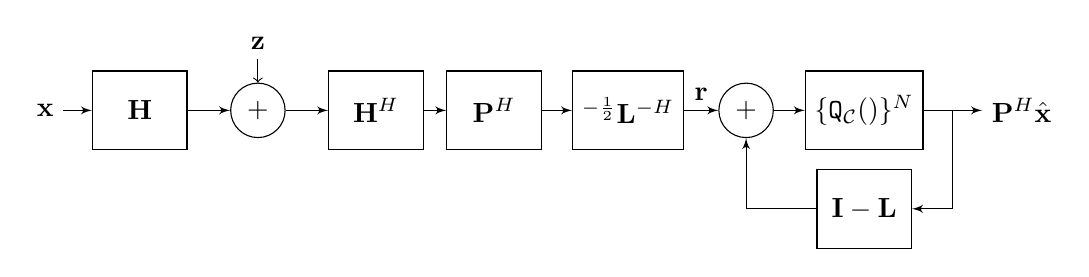
\begin{tikzpicture}[auto, node distance=2cm,>=latex']
        \node [pinstyle] (input)  {$\x$};
        \node [block,right of=input,node distance=1.2cm] (ch) {$\Hb$} ;
        \draw[->] (input) -- (ch);
        \node [sum, right of=ch, node distance=1.5cm, pin={[pinstyle, pin distance=.3cm]above:$\z$}] (sum) {$+$};
        \draw [->] (ch) -- (sum);
        \node [block, right of = sum, node distance=1.5cm] (pf) {$\Hb^H$} ;
        \draw [->] (sum) -- (pf);
        \node [block, right of = pf, node distance=1.5cm] (mf) {$\Pb^H$} ;
        \draw [->] (pf) -- (mf);
        \node [block, right of = mf, node distance=1.7cm] (ff) {$\Deltab^{-\frac{1}{2}}\Lb^{-H}$} ;
        \draw [->] (mf) -- (ff);
        \node [sum, right of=ff, node distance=1.5cm] (sum2) {$+$};
        \draw [->] (ff) -- node {$\rr$} (sum2);
        \node [block, right of = sum2, node distance=1.5cm] (qtz) {$\{\texttt{Q}_{\mathcal{C}}()\}^N$};
        \draw[->] (sum2) -- (qtz);
        \node [pinstyle,right of = qtz,node distance=2cm] (out)  {$\Pb^{H}\hat{\x}$};
        \draw[->] (qtz) -- node [name=tap] {} (out);
        \node [block, below of=qtz, node distance=1.25cm] (feedback) {$\I-\Lb$};
        \draw [->] (tap) |- node [above,pos=0.79] {} (feedback) ;
        \draw [->] (feedback) -| node[pos=0.99] {} node [near end] {} (sum2);
    \end{tikzpicture}
    \end{figure}

    \begin{itemize}
        \item Cholesky decomposition of $\Pb^H\Hb^H\Hb\Pb$ 
        \item Different values $\delta_1\dots\delta_{n_t}$  for each $\Pb$
        \item Optimal $\Pb^*$ NP-Hard combinatorial search
        \begin{itemize}
            \item $\max\min \delta_{i}$ (worst SNR)
            \item $\max \delta_{1}$ (early errors)
            \item $\max \sum \delta_i$ 
        \end{itemize}
    \end{itemize}
    \pagebreak
    
\begin{figure}
    \centering
    \caption{General Linear Receiver with Decision Feedback Block Diagram}
\vspace{-.2in}    
    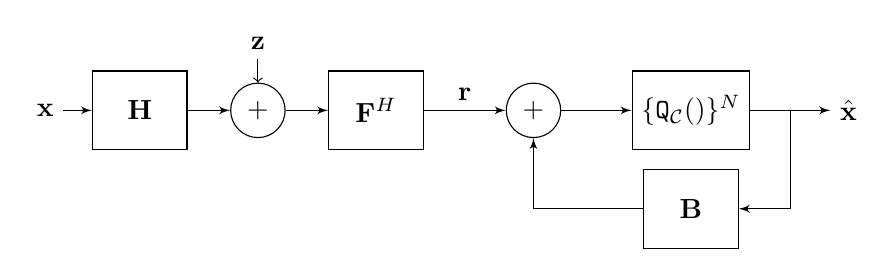
\begin{tikzpicture}[auto, node distance=2cm,>=latex']
        \node [pinstyle] (input)  {$\x$};
        \node [block,right of=input,node distance=1.2cm] (ch) {$\Hb$} ;
        \draw[->] (input) -- (ch);
        \node [sum, right of=ch, node distance=1.5cm, pin={[pinstyle, pin distance=.3cm]above:$\z$}] (sum) {$+$};
        \draw [->] (ch) -- (sum);
        \node [block, right of = sum, node distance=1.5cm] (ff) {$\F^H$} ;
        \draw [->] (sum) -- (ff);
        \node [sum, right of=ff, node distance=2cm] (sum2) {$+$};
        \draw [->] (ff) -- node {$\rr$} (sum2);
        \node [block, right of = sum2, node distance=2cm] (qtz) {$\{\texttt{Q}_{\mathcal{C}}()\}^N$};
        \draw[->] (sum2) -- (qtz);
        \node [pinstyle,right of = qtz,node distance=2cm] (out)  {$\hat{\x}$};
        \draw[->] (qtz) -- node [name=tap] {} (out);
        \node [block, below of=qtz, node distance=1.25cm] (feedback) {$\B$};
        \draw [->] (tap) |- node [above,pos=0.79] {} (feedback) ;
        \draw [->] (feedback) -| node[pos=0.99] {} node [near end] {} (sum2);
    \end{tikzpicture}
    \end{figure}
    \vspace{-.1in}
\begin{columns}[T]
 \begin{column}{6cm}
  \begin{itemize}
     \item Forward Filter $\rr=\F^H\y$\\ \ \\
     \item Feedback Filter $\B^H$\\ \ \\
     \item $\M$ and Cholesky of ZF, MMSE1, or permutations
    \end{itemize}
 \end{column}
 \begin{column}{6cm}
 \begin{table}
  \begin{tabular}{l|cc}
   &$\F^H$&$\B$\\\hline
   MF&$\Hb^H$&$\zero$\\
   ZF&$(\Hb^H\Hb)^{-1}\Hb^H$&$\zero$\\
   MMSE&$(\Hb^H\Hb+\frac{n_t\sigma_z^2}{P}\I)^{-1}\Hb^H$&$\zero$\\
   PIC&$\Hb^H$&$\I-\M$\\
   SIC&$\Deltab^{-\frac{1}{2}}\Q^H$&$\I-\Lb$\\
  \end{tabular}
 \end{table}
 \end{column}
\end{columns}

}

\frame[allowframebreaks]{\frametitle{\small Non-linear MIMO Receivers: Iterative Detection and Decoding}
     \begin{itemize}
          \item IDD is similar to Turbo decoding          
     \begin{figure}
        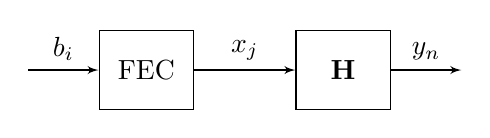
\begin{tikzpicture}[auto, node distance=1.5cm,>=latex']
        \node [input, name=input] {};
        \node [block, right of=input, node distance=1.5cm] (code) {FEC};
        \node [block, right of=code, node distance=2.5cm] (chan) {$\Hb$};
        \node [output, right of=chan, node distance=1.5cm] (output) {};
        \draw [draw,->] (input) -- node {$b_i$} (code);
        \draw [->] (code) -- node {$x_j$} (chan);
        \draw [->] (chan) -- node [name=y] {$y_n$}(output);
        \end{tikzpicture}
    \end{figure}
     \begin{itemize}
          \item Forward Error Correction outer code
          \item Treat channel ISI as inner code\\ \ \\
    \end{itemize}
    \end{itemize}
        
    \begin{itemize}
     \item IDD is an instance of general MAP decoding
    \begin{itemize}
        \item Convolutional, LDPC, Turbo codes...
        \item AKA ``Belief Propagation'' in estimation
        \item AKA ``Message Passing'' in optimization\\ \ \\
    \end{itemize}
     \item MAP criterion $\hat{\bb}=\max_{\bb}f(\y|\bb)f(\bb)$ minimizes error probability
        \begin{itemize}
        \item ML $\hat{\bb}=\max_{\bb}f(\y|\bb)$ optimum if $\bb$ equiprobable\\ \ \\        
        \end{itemize}
        \pagebreak
     \item Scenarios with a chain of random transformations $$\bb\to\x=T_1(\bb)\to\y=T_2(\x)$$
     \item True MAP criterion is $\max_{\bb} f(\y|\x)f(\x|\bb)f(\bb)$
     \item Reduce complexity solving \textit{partial MAP problems} iteratively
        \begin{equation}
            \begin{split}
                \hat{\x}^{(i)}&=\max_{\x} f(\y|\x)\hat{f}^{(i-1)}(\x)\\
                &\;\textnormal{ s.t. } \hat{f}^{(i-1)}(\x)=\sum_{\bb} \hat{f}^{(i-1)}(\x|\bb)f(\bb)
            \end{split}
        \end{equation}

        \begin{equation}
            \begin{split}
                \hat{f}^{(i)}(\x|\bb)=&\arg\max_{\bb} f(\hat{\x}^{(i)}|\bb)f(\bb)\\
            \end{split}
        \end{equation}
        
        
     \item Even if $f(\bb)$ is equiprobable, $\hat{f}^{(i)}(\x)$ \textbf{is not}
        \begin{equation}
            \begin{split}
                \hat{\x}^{(i)}&=\max_{\x} f(\y|\x)\hat{f}^{(i-1)}(\x)\\
                &\;\textnormal{ s.t. } \hat{f}^{(i-1)}(\x)=\frac{1}{B}\sum_{\bb} \hat{f}^{(i-1)}(\x|\bb)
            \end{split}
        \end{equation}

        \begin{equation}
            \begin{split}
                \hat{f}^{(i)}(\x|\bb)=&\arg\max_{\bb} f(\hat{\x}^{(i)}|\bb)\\
            \end{split}
        \end{equation}
     \item \textbf{We can define \textit{partial MAP problems with auxiliar variables} to design iterative decoders even if the global problem is a ML estimation}\\ \ \\
         
     \pagebreak   
     \begin{definition}[Log Likelihood Ratio of BPSK $x_n$ given $y_n$]
        $$\Lambda(x_n|y_n)=\log\frac{P(x_n=1|y)}{P(x_n=-1|y)}=\underset{\textnormal{extrinsic}}{\underbrace{\log\frac{\mathcal{L}_{y_n}(x_n=1)}{\mathcal{L}_{y_n}(x_n=-1)}}}+\underset{\textnormal{apriori}}{\underbrace{\log\frac{P(x_n=1)}{P(x_n=-1))}}}$$      \end{definition}
        \begin{itemize}
          \item If symbols $x_n$ are equiprobable
            $$\frac{P(x_n=1|y_n)}{P(x_n=-1|y_n)}=\frac{P(y_n|x_n=1)}{P(y_n|x_n=-1)}$$
          \item LLRs for non-binary constellations can be defined\\ \ \\
     \pagebreak
          \item MAP can be expressed as max sum\\ \ \\
          \item We can decompose LLRs into \textit{Extrinsic} and \textit{A-priori} parts
        \begin{equation*}
        \small
         \begin{split}
          \max_{b_1\dots b_N}f(\bb|\y)&=\max_{b_1\dots b_N}\prod_{n}f(b_n|\{b_{n'}\}_{n'=1}^{n-1},\y)\\
                                     &=\max_{b_1\dots b_N}\sum_{n}\Lambda(b_n|\y)+\textnormal{consts}\\
                                     &= \max_{b_1\dots b_N}\sum_{n}\Lambda_{E}(b_n|\y)+\sum_{n}\Lambda_{A}(b_n)+\textnormal{consts}
         \end{split}
        \end{equation*}  
          \item Iterative MAP building block at step $(i)$: 
          \begin{columns}
          \begin{column}{5cm}
           \begin{figure}
            \begin{tikzpicture}[scale=.7,transform shape]
             \node[input, inter node distance=2cm] (y) at (0,0){};
             \node[block,right of=y, inter node distance=3cm] (step) {MAP};
             \node[input,below of=step, inter node distance=1cm] (feed){};
             \node[input,below of=feed, inter node distance=.75cm] (fin){};
             \node[sum,right of=step, inter node distance=2cm] (sum){};
             \node[output,right of=step, inter node distance=2cm] (out){};
             \draw[->] (input) -- node[anchor=south] {$\y$} (step);      
             \draw[->] (fin) -- node[anchor=west,pos=.25] {$\Lambda_{A}^{(i-1)}(b_n)$} (step);  
             \draw[->] (feed) -| node[anchor=west,pos=.99]{$-$} (sum);             
             \draw[->] (step) -- (sum);             
             \draw[->] (sum) -- node[anchor=south,pos=.75] {$\Lambda_{E}(b_n|\y)$} (out);             
            \end{tikzpicture}
           \end{figure}
          \end{column}
          \begin{column}{7cm}
            \begin{itemize}
             \item Receive $\Lambda_{A}^{(i-1)}(b_n)$ and $\y$
             \item Calculate $\Lambda^{(i)}(b_n|\y)$
             \item Pass $\Lambda_{E}^{(i)}(b_n|\y)$ to other blocks
            \end{itemize}
          \end{column}
          \end{columns}

          \pagebreak
   
     
     \item Example: Systematic block code $\cc=\left[\I_K;\Pb_{K,N-K}\right]\bb=\left[\bb; \s\right]$        
     \item Tanner Graph (Hamming 4/7)
     \begin{figure}
        \begin{tikzpicture}[scale=.5]         
            \foreach \x in {0,1,...,3} { 
                \node[draw,square] at (3*\x,3){\tiny $b_\x$};
                }
            \foreach \x in {0,1,...,2} { 
                \node[draw,circle] at (1.5+3*\x,0){\tiny $s_\x$};
                }   
                \draw (0,2.5) -- (1.5,.75);
                \draw (3,2.5) -- (1.5,.75);
                \draw (9,2.5) -- (1.5,.75);
                \draw (0,2.5) -- (4.5,.75);
                \draw (6,2.5) -- (4.5,.75);
                \draw (9,2.5) -- (4.5,.75);
                \draw (3,2.5) -- (7.5,.75);
                \draw (6,2.5) -- (7.5,.75);
                \draw (9,2.5) -- (7.5,.75);
        \end{tikzpicture}
     \end{figure}
        \item Direct part: $\textcolor{KYJade}{\Lambda_E^{(i)}(y_{_{1\dots K}}|\bb)}\leftarrow \max_{\bb} \Lambda^{(i)}(y_{_{1\dots K}}|\bb)\textnormal{ s.t. }\textcolor{VCobalt}{\Lambda_{A|y_{_{K+1\dots N}}}^{(i-1)}(\bb)}$
        \item Parity check: $\textcolor{VCobalt}{\Lambda_E^{(i)}(y_{_{K+1\dots N}}|\bb)}\leftarrow \max_{\bb} \Lambda^{(i)}(y_{_{K+1\dots N}}|\bb)\textnormal{ s.t. }\textcolor{KYJade}{\Lambda_{A|y_{_{1\dots K}}}^{(i-1)}(\bb)}$\\ \ \\
        \item \textbf{Parrallel} $y_{_{1\dots K}}=T_1(\bb)$ and $y_{_{K+1\dots N}}=T_2(\s)=T_2(\Pb\bb)$\\ \ \\
        \item  $\hat{f}^{(i)}(\bb|y_{_{1\dots K}})$ and $\hat{f}^{(i)}(\bb|y_{_{K+1\dots N}})$ not equip. even if $f(\bb)$ is
        
    \end{itemize}   
          
          \pagebreak
          \item Consider the notation
          $$y_i=h_{i,i}x_{i}+\underset{\xi_j}{\underbrace{\sum_{j\neq i}h_{i,j}x_{j}}}+z_i$$
          \item Initialization:          
            \begin{itemize}
             \item Detector computes initial $\Lambda^{(0)}(x_i|y_i)$ with assumption 
          $$\sum_{i\neq j}h_{j,i}x_{m}+z_n\approx\mathcal{N}(0,\mathrm{Var}(\xi_n)+\sigma^2_z)$$
            \item Interference variance is computed as
                $$\mathrm{Var}(\xi_n)=\sum_{m\neq n}|h_{n,m}|^2\mathrm{Var}(x_{m})$$          
                $$\mathrm{Var}(x_{m})=1-(P(x_m=1)-P(x_m=-1))^2$$
            \end{itemize}
            \pagebreak
            
            
    \begin{center}
        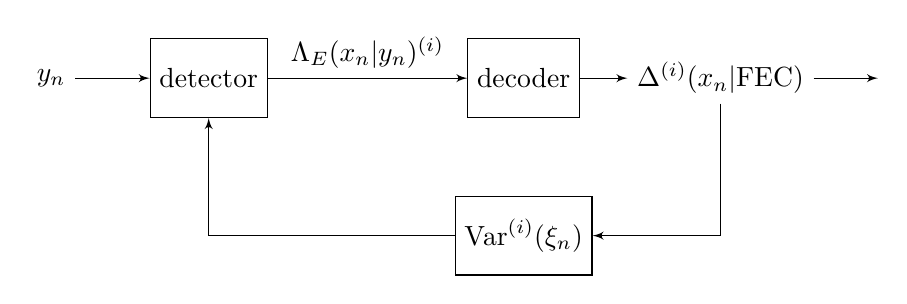
\begin{tikzpicture}[auto, node distance=2cm,>=latex']
        \node [pinstyle, name=input] {$y_n$};
        \node [block, right of=input] (dete) {detector};
        \node [block, right of=dete, node distance=4cm] (deco) {decoder};
        \node [pinstyle, right of=deco, node distance=2.5cm] (llr) {$\Delta^{(i)}(x_n|\mathrm{FEC})$};
        \node [output, right of=llr] (output) {};
        \node [block, below of=deco] (feedback) {$\mathrm{Var}^{(i)}(\xi_n)$};
        \draw [draw,->] (input) -- node {} (dete);
        \draw [->] (dete) -- node {$\Lambda_E(x_n|y_n)^{(i)}$} (deco);
        \draw [->] (deco) -- (llr);
        \draw [->] (llr) -- (output);
        \draw [->] (llr) |-  (feedback) ;
        \draw [->] (feedback) -| node[pos=0.99] {} node [near end] {} (dete);
        \end{tikzpicture}
    \end{center}
          \item For $i=1$ to Max. Num. Iterations
    \begin{itemize}
            \item FEC decoder: Compute $\Delta^{(i)}(x_n|\mathrm{FEC})$ with a priori $\Lambda(x_n|y_n)^{i-1}$ \\ \ \\
            \item Feedback: recalculate $\mathrm{Var}^{(i)}(\xi_n)$ using $\Delta_{E}^{(i)}(x_n|\mathrm{FEC})$\\ \ \\
            \item MIMO detector: Compute $\Lambda^{(i)}(x_n|y_n)$ with a priori $\mathrm{Var}^{(i)}(\xi_n)$\\ \ \\
    \end{itemize}
          \item Output: A Posteriori Probabilities $\Lambda(b_n|\y)$ (soft decision)
    \end{itemize}
}

\end{document}


